\documentclass[leqno, openany]{memoir}
\setulmarginsandblock{3.5cm}{3.5cm}{*}
\setlrmarginsandblock{3cm}{3.5cm}{*}
\checkandfixthelayout

\usepackage{amsmath}
\usepackage{amssymb}
\usepackage{amsthm}
%\usepackage{MnSymbol}
\usepackage{bm}
\usepackage{accents}
\usepackage{mathtools}
\usepackage{tikz}
\usetikzlibrary{calc}
\usetikzlibrary{automata,positioning}
\usepackage{tikz-cd}
\usepackage{forest}
\usepackage{braket} 
\usepackage{listings}
\usepackage{mdframed}
\usepackage{verbatim}
\usepackage{physics}
\usepackage{spectralsequences} 
\usepackage{stackengine}
%\usepackage{/home/patrickl/homework/macaulay2}

%font
\usepackage[osf]{mathpazo}
\usepackage{microtype}

%CS packages
\usepackage{algorithmicx}
\usepackage{algpseudocode}
\usepackage{algorithm}

% typeset and bib
\usepackage[english]{babel} 
\usepackage[utf8]{inputenc} 
\usepackage[backend=biber, style=alphabetic]{biblatex}
\usepackage[bookmarks, colorlinks, breaklinks]{hyperref} 
\hypersetup{linkcolor=black,citecolor=black,filecolor=black,urlcolor=black}

% other formatting packages
\usepackage{float}
\usepackage{booktabs}
\usepackage{enumitem}
\usepackage{csquotes}
\usepackage{titlesec}
\usepackage{titling}
\usepackage{fancyhdr}
\usepackage{lastpage}
\usepackage{parskip}

\usepackage{lipsum}

% delimiters
\DeclarePairedDelimiter{\gen}{\langle}{\rangle}
\DeclarePairedDelimiter{\floor}{\lfloor}{\rfloor}
\DeclarePairedDelimiter{\ceil}{\lceil}{\rceil}


\newtheorem{thm}{Theorem}[section]
\newtheorem{cor}[thm]{Corollary}
\newtheorem{prop}[thm]{Proposition}
\newtheorem{lem}[thm]{Lemma}
\newtheorem{conj}[thm]{Conjecture}
\newtheorem{quest}[thm]{Question}

\theoremstyle{definition}
\newtheorem{defn}[thm]{Definition}
\newtheorem{defns}[thm]{Definitions}
\newtheorem{con}[thm]{Construction}
\newtheorem{exm}[thm]{Example}
\newtheorem{exms}[thm]{Examples}
\newtheorem{notn}[thm]{Notation}
\newtheorem{notns}[thm]{Notations}
\newtheorem{addm}[thm]{Addendum}
\newtheorem{exer}[thm]{Exercise}

\theoremstyle{remark}
\newtheorem{rmk}[thm]{Remark}
\newtheorem{rmks}[thm]{Remarks}
\newtheorem{warn}[thm]{Warning}
\newtheorem{sch}[thm]{Scholium}


% unnumbered theorems
\theoremstyle{plain}
\newtheorem*{thm*}{Theorem}
\newtheorem*{prop*}{Proposition}
\newtheorem*{lem*}{Lemma}
\newtheorem*{cor*}{Corollary}
\newtheorem*{conj*}{Conjecture}

% unnumbered definitions
\theoremstyle{definition}
\newtheorem*{defn*}{Definition}
\newtheorem*{exer*}{Exercise}
\newtheorem*{defns*}{Definitions}
\newtheorem*{con*}{Construction}
\newtheorem*{exm*}{Example}
\newtheorem*{exms*}{Examples}
\newtheorem*{notn*}{Notation}
\newtheorem*{notns*}{Notations}
\newtheorem*{addm*}{Addendum}


\theoremstyle{remark}
\newtheorem*{rmk*}{Remark}

% shortcuts
\newcommand{\Ima}{\mathrm{Im}}
\newcommand{\A}{\mathbb{A}}
\newcommand{\N}{\mathbb{N}}
\newcommand{\R}{\mathbb{R}}
\renewcommand{\H}{\mathbb{H}}
\newcommand{\C}{\mathbb{C}}
\newcommand{\Z}{\mathbb{Z}}
\newcommand{\F}{\mathbb{F}}
\newcommand{\Q}{\mathbb{Q}}
\renewcommand{\k}{\Bbbk}
\renewcommand{\P}{\mathbb{P}}
\newcommand{\M}{\overline{M}}
\newcommand{\g}{\mathfrak{g}}
\newcommand{\h}{\mathfrak{h}}
\newcommand{\n}{\mathfrak{n}}
\renewcommand{\b}{\mathfrak{b}}
\newcommand{\ep}{\varepsilon}
\newcommand*{\dt}[1]{%
   \accentset{\mbox{\Huge\bfseries .}}{#1}}
\renewcommand{\abstractname}{Official Description}
\newcommand{\mc}[1]{\mathcal{#1}}
\newcommand{\T}{\mathbb{T}}
\newcommand{\mf}[1]{\mathfrak{#1}}
\newcommand{\mr}[1]{\mathrm{#1}}
\newcommand{\ms}[1]{\mathsf{#1}}
\newcommand{\ol}[1]{\overline{#1}}
\newcommand{\wt}[1]{\widetilde{#1}}
\newcommand{\wh}[1]{\widehat{#1}}

\DeclareMathOperator{\Der}{Der}
\DeclareMathOperator{\Sq}{Sq}
\DeclareMathOperator{\Hom}{Hom}
\DeclareMathOperator{\colim}{colim}
\DeclareMathOperator{\coker}{coker}
\DeclareMathOperator{\End}{End}
\DeclareMathOperator{\ad}{ad}
\DeclareMathOperator{\Aut}{Aut}
\DeclareMathOperator{\Rad}{Rad}
\DeclareMathOperator{\supp}{supp}
\DeclareMathOperator{\sgn}{sgn}
\DeclareMathOperator{\spec}{Spec}
\DeclareMathOperator{\Vect}{Vect}

% Section formatting
\titleformat{\section}
    {\Large\sffamily\scshape\bfseries}{\thesection}{1em}{}
\titleformat{\subsection}[runin]
    {\large\sffamily\bfseries}{\thesubsection}{1em}{}
\titleformat{\subsubsection}[runin]{\normalfont\itshape}{\thesubsubsection}{1em}{}

\title{COURSE TITLE}
\author{Lectures by INSTRUCTOR, Notes by NOTETAKER}
\date{SEMESTER}

\newcommand*{\titleSW}
    {\begingroup% Story of Writing
    \raggedleft
    \vspace*{\baselineskip}
    {\Huge\itshape Algebraic Topology \\ Spring 2021}\\[\baselineskip]
    {\large\itshape Notes by Patrick Lei}\\[0.2\textheight]
    {\Large Lectures by Francesco Lin}\par
    \vfill
    {\Large \sffamily Columbia University}
    \vspace*{\baselineskip}
\endgroup}
\pagestyle{simple}

\chapterstyle{ell}


%\renewcommand{\cftchapterpagefont}{}
\renewcommand\cftchapterfont{\sffamily}
\renewcommand\cftsectionfont{\scshape}
\renewcommand*{\cftchapterleader}{}
\renewcommand*{\cftsectionleader}{}
\renewcommand*{\cftsubsectionleader}{}
\renewcommand*{\cftchapterformatpnum}[1]{~\textbullet~#1}
\renewcommand*{\cftsectionformatpnum}[1]{~\textbullet~#1}
\renewcommand*{\cftsubsectionformatpnum}[1]{~\textbullet~#1}
\renewcommand{\cftchapterafterpnum}{\cftparfillskip}
\renewcommand{\cftsectionafterpnum}{\cftparfillskip}
\renewcommand{\cftsubsectionafterpnum}{\cftparfillskip}
\setrmarg{3.55em plus 1fil}
\setsecnumdepth{subsection}
\maxsecnumdepth{subsection}
\settocdepth{subsection}

\begin{document}
    
\begin{titlingpage}
\titleSW
\end{titlingpage}

\thispagestyle{empty}
\section*{Disclaimer}%
\label{sec:disclaimer}

These notes were taken during lecture using the \texttt{vimtex} package of the editor \texttt{neovim}. 
Any errors are mine and not the instructor's. 
In addition, my notes are picture-free (but will include commutative diagrams) and are a mix of my mathematical style and that of the instructor.
If you find any errors, please contact me at \texttt{plei@math.columbia.edu}.
\newpage


\tableofcontents

\chapter{Spectral Sequences}%
\label{cha:spectral_sequences}

Our goal in this chapter will be to compute the homotopy groups of spheres, but we are not algebraic topologists so we don't actually care about that. What we know from the basic theory is that $\pi_i(S^n) = 0$ if $i < n$ and $\pi_n(S^n) = \Z$, and this isomorphism is given by the degree. We also know that $\pi_3(S^2) = \Z$ and is generated by the Hopf fibration $S^1 \hookrightarrow S^3 \to S^2$. Note that this map is the attaching map of the $4$-cell of $\C\P^2$.

There is an analogous decomposition $\H\P^2 = \mr{pt} \cup D^4 \cup D^8$. Then we obtain a fibration $f \colon S^7 \to S^4$, which is an $S^3$-fibration. Using the long exact sequence of the fibration, we see that $\pi_7(S^4) \supseteq \Z$.

Next, we may consider $\mathbb{O}\P^2$, the octonionic projective plane. This has a cell decomposition $\mr{pt} \cup D^8 \cup D^{16}$ and from this we obtain a fibration $S^7 \hookrightarrow S^{15} \to S^8$ and compute that $\pi_{15}(S^8) \supseteq \Z$. We should note, however, that $\mathbb{O}\P^2$ is \textbf{not} the set of lines in $\mathbb{O}^3$ because the octonions do not form an associative algebra. There is enough associativity to define some sort of $\mathbb{O}\P^2$ but not $\mathbb{O}\P^n$ for $n \geq 3$. In fact, we will prove that no space with the expected cohomology ring exists.

More generally, we can study $f \colon S^{2n-1} \to S^n$ as follows: Consider the mapping cone $S^n \cup_f D^{2n} \eqqcolon C_f$. Then the cohomology is
\[ H^i(C_f) = \begin{cases}
    \Z & i = 0, n, 2n \\
    0 & \text{otherwise}
\end{cases}. \]
Then choose generators $\alpha \in H^n, \beta \in H^{2n}$. We then have $\alpha^2 = H(f) \beta \in H^{2n}$ for some integer $H(f)$, called the \textit{Hopf invariant}.

\begin{exm}
    The attaching maps of $\C\P^2, \H\P^2, \mathbb{O}\P^2$ all have $H(f) = 1$. This implies that $H^* = \Z[\alpha]/(\alpha^3)$.
\end{exm}

We know that if $f,g$ are homotopic, then $H(f) = H(g)$ because the mapping cones are homotopy equivalent. Then we obtain a homomorphism $H \colon \pi_{2n-1}(S^n) \to \Z$. Note that when $n$ is odd, we have $\alpha^2 = -\alpha^2$ by graded commutativity, and so $H(f) = 0$.

\begin{exm}
    If $n = 2k$ is even, there exists $f \colon S^{4k-1} \to S^{2k}$ with $H(f) = 2$.
\end{exm}

Now given a pointed space $(X,e)$ define $J_2(X) = X \times X / (x,e) \sim (e,x)$. This is somewhere between the product and the smash product, and so $J_2(S^{2k})$ is a CW complex with a single cell in dimensions $0, 2k, 4k$.

\begin{exer}
    The attaching map of the $4k$-cell has $H(f) = 2$.
\end{exer}

\begin{cor}
    $\pi_{4k-1}(S^{2k})$ admits a $\Z$-summand. This is because $H$ surjects onto either $2\Z$ or $\Z$, and so it splits.
\end{cor}

We have the following results:

\begin{thm}[Serre]
    $\pi_i(S^n)$ is a finitely generated abelian group. It has rank $1$ if $i = n$ or $i = 2n-1$ and $n$ is even.
\end{thm}

\begin{thm}[Adams]
    If $[f] \in \pi_{2n-1}(S^n)$ with $H(f) = 1$, then $n = 2,4,8$.
\end{thm}

\begin{rmk}
    This is related to the following. Suppose $\R^n$ admits the structure of a division algebra. This is a bilinear map $* \colon \R^n \otimes \R^n \to \R^n$ that is invertible for $a \neq 0$. Then $n = 1,2,4,8$. We will prove this result using K-theory.
\end{rmk}

\section{The Simplest Case}%
\label{sec:the_simplest_case}

Here, we will consider $\pi_{n+1}(S^n)$ for $n \geq 3$. By the Freudenthal suspension theorem, we have maps
\[ \pi_3(S^2) \xrightarrow{\Sigma} \pi_4(S^3) \xrightarrow[\sim]{\Sigma} \pi_5(S^4) \to \cdots \]
Therefore the group we need to compute is $\pi_4(S^3)$. The key strategy is to exploit the interaction between homotopy and homology. Here, we will consider the \textit{Hurewicz map}
\[ h \colon \pi_n(X) \to H_n(X) \qquad [f] \mapsto f_* [S^n]. \]

\begin{thm}[Hurewicz]
    Suppose $n \geq 2$ and $X$ is $(n-1)$-connected. Then $\wt{H}_0(X) = H_1(X) = \cdots = H_{n-1}(X) = 0$ and $h \colon \pi_n(X) \simeq H_n(X)$.
\end{thm}

\begin{rmks}
    When $n = 1$, $H_1(X)$ is the abelianization of $\pi_1(X)$. Also, there is a relative version of the Hurewicz theorem.
\end{rmks}

\begin{proof}[Sketch of Proof]
    We can assume $X$ is a CW complex with a single $0$-cell and no cells in dimension $1, \ldots, n-1$. Then we can replace $X$ with $X^{n+1}$, so we can write
    \[ X = \qty( \bigvee_{\alpha} S_{\alpha}^n ) \cup_{\beta} D_{\beta}^{n+1}. \]
    By homotopy excision, we have
    \[ \pi_n(X) = \mr{coker}(d \colon \pi_{n+1}(X, X^n) \to \pi_n(X^n)) \]
    and this is exactly $C_{n+1}(X) \to C_n(X) \to 0$.
\end{proof}

Our strategy to compute $\pi_4(S^3)$ will be to construct a space whose homology is $\pi_4(S^3)$. Recall that $\pi_3(K(\Z, 3)) = \Z$ by definition, and so consider $f \colon S^3 \to K(\Z, 3)$ be a generator. Then $f_* \colon \pi_3(S^3) \xrightarrow{\sim} \pi_3(K(\Z, 3))$ is an isomorphism. Now we can turn $f$ into a fibration $F \hookrightarrow S^3 \to K(\Z, 3)$. Considering the long exact sequence of the fibration, we have
\[ 0 \to \pi_4(F) \to \pi_4(S^3) \to 0 \to \pi_3(F) \to \pi_3(S^3) \to \pi_3(K(\Z, 3)) \to \cdots \]
and therefore $\pi_0(F) = \pi_1(F) = \pi_2(F) = \pi_3(F) = 0$. We also have $\pi_n(F) \cong \pi_n(S^3)$ for $n \geq 4$. In particular, we have $\pi_4(S^3) = \pi_4(F) = H_4(F)$.If we can understand $F$ in some reasonable way, then we will be done.

If we turn $F \hookrightarrow S^3$ into a fibration, then the homotopy fiber is now a $K(\Z, 2) = \C\P^{\infty}$. Now we have a fibration and we know the homology of both $S^3$ and $\C\P^{\infty}$, so the question is to compute $H_4$ from the information we have.

\begin{quest}
    Given $F \hookrightarrow E \to B$ a fibration, is there a relationship between $H_*(B), H_*(E), H_*(F)$?
\end{quest}

Recall that in the case when $E \cong F \times B$ this relation is given by the K\"unneth formula. Here, we see that $C_*(E) = C_*(F) \otimes C_*(B)$ as chain complexes, and so we reduce the problem to homological algebra. This gives us

\begin{thm}
    Let $R$ be a principal ideal domain. Then there is a natural short exact sequence
    \[ 0 \to \bigoplus H_i(F,R) \otimes H_{n-i}(B, R) \to H_n(F \times B, R) \to \bigoplus \mr{Tor}^1_R(H_i(F,R), H_{n-1-i}(B, R)) \to 0 \]
    and this sequence splits (but not naturally).
\end{thm}

\begin{exm}
    We can compute that $H_*(S^1 \times S^2) = \Z$ in dimensions $0,1,2,3$.
\end{exm}

However, we note that the Kunneth theorem does not hold for fibrations in general. To see this, consider the Hopf fibration.

\begin{exm}
    Consider the fibration $K(\Z, n-1) \hookrightarrow * \to K(\Z, n)$. Both the base and fiber have nontrivial homology, but clearly the total space is contractible, so it has trivial homology. In both examples, $H_*(E)$ is \textbf{smaller} than what we would get from K\"unneth. 
\end{exm}

\section{Spectral Sequences}%
\label{sec:spectral_sequences}

\begin{defn}
    A \textit{spectral sequence} is a sequence $(E^r, d_r)$, where $E^r$ is an $R$-module and $d_r \colon E^r \to E^r$ is a differential. In addition, we require that $E^{r+1} = H_*(E^r, d_r)$. 
\end{defn}

\begin{rmk}
    Note that $(E^r, d_r)$ determines $E^{r+1}$, but not $d_{r+1}$ in general.
\end{rmk}

Now assume that $d_r = 0$ for $r \gg 0$ so that $E^r = E^{r+1} = \cdots \eqqcolon E^{\infty}$.

\begin{defn}
    We say that $(E^r, d_r) \Rightarrow G$, or $(E_r, d_r)$ \textit{converges to $G$}, if $G$ admits a filtration
    \[ 0 = G_{-1} \subset G_0 \subset G_1 \subset \cdots \subset G_n = G \] such that $\bigoplus G_i / G_{i-1} \cong E^{\infty}$.
\end{defn}

\begin{rmk}
    This says that $G$ is recovered by $(E^r, d_r)$ up to extension problems.
\end{rmk}

\begin{exm}
    Consider a short exact sequence $0 \to A_* \to C_* \to C_*/A_* \to 0$ of chain complexes. Then we will see that there is a spectral sequence with $E^1 = H_*(A) \oplus H_*(C/A)$ and $(E^r, d_r) \Rightarrow H_*(C)$. 

    First, consider the long exact sequence in homology. If we consider the boundary homomorphism $\delta_i$, we obtain a long exact sequence
    \[ 0 \to \operatorname{coker} \delta_{i+1} \to H_i(C) \to \ker \delta_i \to 0. \]
    Now define $E^1 = H_*(A) \oplus H_*(C / A)$ with $d_1 = \bigoplus \delta_i$. Then we have 
    \[ H_*(E^1, d_1) = \qty( \bigoplus \ker \delta_i ) \oplus \qty(\bigoplus \operatorname{coker} \delta_i) \eqqcolon E^2, \]
    as desired. Then we let $d_2 = 0$.
\end{exm}

This tells us that if $H_*(A) = H_*(C/A) = 0$, then $H_*(C) = 0$. Also, if $H_*(C) = 0$, then $H_*(A) \cong H_*(C/A)$ with a shift.

\begin{thm}[Serre]
    Let $F \hookrightarrow E \to B$ be a fibration and let $\pi_1(B) = 1$. Then there is a spectral sequence $(E^r, d_r)$ such that
    \begin{itemize}
        \item $E^2 \cong H_*(B; H_*(F))$;
        \item $(E^r, d_r) \Rightarrow H_*(E)$.
    \end{itemize}
\end{thm}

Note here that we need to define what it means to converge in this setting. Also, note that $E^3$ is smaller than $E^2$, so this formalizes the notion that $H_*(E)$ is smaller than what we naively expect.

\begin{rmk}
    We actually do not know what $d_2$ is, so it is impossible to compute the homology in general.
\end{rmk}

Fortunately, there is more structure:
\begin{itemize}
    \item $E^r_{*,*}$ is bigraded.
    \item $d_r$ has bidegree $(-r, r-1)$.
    \item $E_{p,q}^2 = H_p(B; H_q(F))$.
    \item $E_{p,q}^r = E_{p,q}^{\infty}$ for $r \gg 0$ depending on $p,q$.
    \item $H_n(E)$ has a filtration with associated graded $\bigoplus E_{i, n-i}^{\infty}$.
\end{itemize}

\begin{exm}
    Consider the example $S^1 \hookrightarrow * \to \C\P^{\infty}$. Then we know that $E_{p,q}^2 = H_p(B, H_q(S^1))$ and therefore the spectral sequence is
    \begin{center}
    \begin{sseqdata}[classes={draw=none},name=cpinf,homological Serre grading,xscale=1.8, y axis gap = 2em]
        \class["H_0(B)"](0,0)
        \class["H_1(B)"](1,0)
        \class["H_2(B)"](2,0)
        \class["H_3(B)"](3,0)
        \class["\ldots"](4,0)
        \class["H_0(B)"](0,1)
        \class["H_1(B)"](1,1)
        \class["H_2(B)"](2,1)
        \class["H_3(B)"](3,1)
        \class["\ldots"](4,1)
        \d[->]2(2,0)
        \d[->]2(3,0)
        \d[->]2(4,0)
    \end{sseqdata}
    \printpage[name=cpinf,page=2, grid=chess]
    \end{center}
    This gives us $\delta_i \colon H_{2+i}(B) \to H_i(B)$, and so $d_3$ has degree $(-3, 2)$ and thus it has to be zero. By degree reasons, we see that $E^4 = E^3$ and $d_4 = 0$, so $E^{\infty} = E^3$. Then, the total space is a point, and so writing the $E^3$-page
    \begin{center}
        \begin{sseqdata}[classes={draw=none},name=cpinf3,homological Serre grading,xscale=1.8, y axis gap = 2em]
            \class["\coker \delta_0"](0,1)
            \class["\coker \delta_1"](1,1)
            \class["\coker \delta_2"](2,1)
            \class["H_0(B)"](0,0)
            \class["H_1(B)"](1,0)
            \class["\ker \delta_0"](2,0)
            \class["\ker \delta_1"](3,0)
            \class["\ker \delta_2"](4,0)
        \end{sseqdata}
        \printpage[name=cpinf3, page=3, grid=chess]
    \end{center}
    we see that $H_0(B) = \Z, H_1(B) = 0$ and that $\ker \delta_i = \operatorname{coker} \delta_i = 0$. This recovers the usual computation of the homology of $\C\P^{\infty}$.
\end{exm}

\begin{exm}
    We want to compute $H_*(\Omega S^2)$. Here, we will use the fiber sequence $\Omega S^2 \hookrightarrow * \to S^2$. Here, we know that $E_{p,q}^2 = H_p(S^2, H_q(F))$, so the $E^2$-page looks like
    \begin{center}
        \begin{sseqdata}[classes={draw=none}, name=omegas2, homological Serre grading, xscale=1.5, y axis gap = 2em]
            \class["H_0(F)"](0,0)
            \class["H_1(F)"](0,1)
            \class["H_2(F)"](0,2)
            \class["H_3(F)"](0,3)
            \class["H_0(F)"](2,0)
            \class["H_1(F)"](2,1)
            \class["H_2(F)"](2,2)
            \class["H_3(F)"](2,3)
            \d["g_0", ->]2(2,0)
            \d["g_1", ->]2(2,1)
            \d["g_2", ->]2(2,2)
        \end{sseqdata}
        \printpage[name=omegas2, page=2, grid=chess]
    \end{center}
    Then the $E^3$-page looks like
    \begin{center}
        \begin{sseqdata}[classes={draw=none}, name=omegas23, homological Serre grading, xscale=1.5, y axis gap = 2em]
            \class["H_0(F)"](0,0)
            \class["\coker g_0"](0,1)
            \class["\coker g_1"](0,2)
            \class["\coker g_2"](0,3)
            \class["\ker g_0"](2,0)
            \class["\ker g_1"](2,1)
            \class["\ker g_2"](2,2)
            \class["\ker g_3"](2,3)
        \end{sseqdata}
        \printpage[name=omegas23, page=3, grid=chess]
    \end{center}
    and the differential has degree $(-3,2)$, so $d_3 = 0$. This implies that $E^{\infty} = E_3$, and so the associated graded pieces are $\Z,0,0,0$. We see that $H_0(F) = \Z$ and each $g_i$ is an isomorphism. This tells us that $H_i(\Omega S^2) \cong \Z$ for all $i$.
\end{exm}

\begin{exm}
    We can enhance this example to $\Omega S^n \hookrightarrow * \to S^n$. In this case, the first possible nontrivial differential is $d_n$, which has degree $(-n, n-1)$. This gives us $E^{n+1} = E^{\infty}$ for degree reasons, so we can compute
    \[ H_i(\Omega S^n) = \begin{cases}
        \Z & (n-1) \mid i \\
        0 & \text{otherwise}.
    \end{cases} \]
    because $\delta_i \colon H_i(F) \to H_{i+n-1}(F)$ is an isomorphism.
\end{exm}

Recall that our goal was to study $\C\P^{\infty} \hookrightarrow F \to S^3$. However, we cannot compute this yet, so we will need to introduce even more structure. To do this, we will need to do some homological algebra.

Considered a filtered chain complex, which is an abelian group $C$ with a map $d \colon C \to C$ such that $d^2 = 0$. To this, we attach a filtration $0 = F_{-1} C \subseteq F_0 C \subseteq \cdots \subseteq F_n C = C$ such that $d(F_i C) \subseteq F_i C$.

\begin{rmk}
    $(F_i C, D)$ is a subcomplex of $C$.
\end{rmk}

Now if $X$ is a topological space with filtration $X_{-1} = \emptyset \subset X_0 \subset \cdots \subset X_n = X$. Then if $C_*(X)$, we can choose $F_i C = C_*(X_i)$, and this is a filtration.

Given $(C,d)$ and a filtration, we can associate two objects:
\begin{enumerate}
    \item $\mr{Gr}_* C = \bigoplus F_i C / F_{i-1} C$, the \textit{associated graded} complex. Then we may consider the homology of this complex, which is a graded object.
    \item Given a subcomplex $(F_i C, d) \hookrightarrow (C,d)$, we have a map $H(F_i C, d) \to H(C, d)$. The image of this is $F_i H(C,d)$, so we get a filtration on the homology $H(C)$. So then we obtain a graded
        \[ \mr{Gr}_* H(C,d) = \bigoplus F_i H(C) / F_{i-1} H(C). \]
\end{enumerate}
Now we want to consider therelationship between the two. Note that the first one is bigger, because $x \in \mr{Gr}_i C$ is a cycle if $\dd{x} \in F_{i-1} C$, while $x \in C$ is a cycle if $\dd{x} = 0$.

\begin{thm}[Leray]
    There exists a spectral sequence $(E_*^r, d_r)$ such that
    \begin{itemize}
        \item $E_*^1 \cong H_* (\mr{Gr}_* C, d_0)$.
        \item The spectral sequence converges to $H(C)$, or more precisely, $E_*^{\infty} \cong \mr{Gr}_* H(C)$.
    \end{itemize}
\end{thm}

\begin{proof}
    Consider the group
    \[ E_p^r = \frac{F_p C \cap \dd^{-1}(F_{p-r} C)}{(F_{p-1} C \cap \dd^{-1} F_{p-r} C) + (F_p C \cap \dd(F_{q+r-1} C))}. \]
    Notice that
    \begin{align*}
        E_p^0 &= \frac{F_p C}{F_{p-1} C + d(F_{p-1} C)} = \frac{F_p C}{F_{p-1} C} \\
        E_p^1 &= \frac{F_p C \cap d^{-1} F_{p-1} C}{F_{p-1}C + d(F_p C)} = H_p(\mr{Gr}_* C, \dd_0) \\
        E_p^{\infty} &= \frac{F_p C \cap \ker \dd}{(F_{p-1} \cap \ker d) + (F_p C \cap \Im d)} = \frac{F_p H(C)}{F_{p-1} H(C)},
    \end{align*}
    so all the groups are as expected. For the differential, we define $\dd{r} \colon E_*^r \to E_r^*$ and in fact $\dd_r \colon E_p^r \to E_{p-r}^r$ and thus has degree $-r$. Choose $\alpha \in E_p^r$ and choose $a \in F_p C \cap \dd^{-1}(F_{p-r} C)$ a representative. Then $\dd{\dd{a}} = 0$ implies that $\dd{a} \in \dd^{-1}(0) \subset \dd^{-1}(F_{p-2r} C)$ and therefore $\dd{a} \in F_{p-r} C \cap d^{-1}(F_{p-2r} C)$. Therefore $\dd{a}$ defines an element in $E_{p-r}^r$, so we set $\dd^r \alpha = [\dd{a}] \in E_{p-r}^r$.

    The things that need to be checked are that this is well-defined, ${(\dd^r)}^2 = 0$, and that $H_*(E_*^r, \dd{r}) \cong E_*^{r+1}$ canonically. All of this is painful homological algebra and is omitted.
\end{proof}

However, we will need something even more painful. Now we will considered a filter graded chain complex $(C_*, \dd)$, where $\dd$ has degree $-1$. Now for a filtration, we can consider the bigraded
\[ \mr{Gr}_{*,*} = \bigoplus_{p,m} \frac{F_p C_m}{F_{p-1} C_m}. \]
Also, we note that $H_m(C)$ is naturally filtered with $F_p H_m(C) = \Im(H_m (F_p C) \to H_m(C))$.

\begin{thm}[Leray]
    There is a spectral sequence $(E_{*,*}^r, \dd{r})$ such that
    \begin{itemize}
        \item $E^1_{*,*} \cong H_{*,*}(\mr{Gr} C)$.
        \item The spectral sequence converges to $H(C)$, where
            \[ E_{p,q}^{\infty} = \frac{F_p H_{p+q}(C)}{F_{p-1}H_{p+q}(C)}. \]
    \end{itemize}
\end{thm}

\begin{proof}
    We write
    \[ E_{p,q}^r = \frac{F_p C_{p+q} \cap \dd^{-1} (F_{p-r} C_{p+q-1})}{[F_{p-1} C_{p+q} \cap \dd^{-1}(F_{p-q}C_{p+q-1})] + [F_p C_{p+q} \cap \dd(F_{p+r-1} C_{p+q+1})]}. \]
    The differential has degree $(-r, r-1)$. Note that it decreases the filtration by $r$ and the total degree by $1$. For $\alpha \in E_{p,q}^r$, choose a representative $a \in F_p C_{p+q}$ with $\dd{a} \in F_{p-r} C_{p+q-1}$. Then $\dd^2 a = 0$ and therefore $\dd{a} \in \dd^{-1}(0) \subseteq \dd^{-1}(F_{p-2r} C_{p+q-1})$, so we set $\dd^r \alpha = [\dd{a}] \in E_{p-r, q+r-1}^r$.
\end{proof}

Returning to topology, consider a filtration $\emptyset = X_{-1} \subseteq X_0 \subseteq \cdots \subseteq X_n = X$, which givs a filtration on $C_*(X)$. This now defines a spectral sequence by setting $F_p C_{p+q}(X) = C_{p+q}(X_p)$. The $E^0$ page of this is simply
\[ E_{p,q}^0 = \frac{F_p C_{p+q}}{F_{p-1} C_{p+q}} = \frac{C_{p+q}(X_p)}{C_{p+q}(X_{p-1})} = C_{p+q}(X_p, X_{p-1}) \]
and $d_{p,q}^0$ is $\partial \colon C_{p+1} \to C_{p+q-1}$.

The $E^1$-page of the spectral sequence is
\[ E^1_{p,q} = H_{p+q}(X_p, X_{p-1})\] 
and $d^1 \colon H_{p+1}(X_p, X_{p-1}) \to H_{p+q-1}(X_{p-1}, X_{p-2})$ is the connecting homomorphism for the triple $(X_p, X_{p-1}, X_{p-2})$. 

The $E^{\infty}$-page of the spectral sequence is
\[ E_{p,q}^{\infty} = \frac{\Im(H_{p+q}(X_p) \to H_{p+q}(X))}{\Im(H_{p+1}(X_{p-1}) \to H_{p+1}(X))}, \]
which is the associated graded of $H_{p+q}(X)$ for the filtration $X_p \hookrightarrow X$.

\begin{exm}
    Consider the cellular homology of $X$. Set $X_p = X^p$, the $p$-skeleton. Then we note that $E_{p,q}^1$ is the homology $H_{p+1}(X_p, X_{p-1})$, and now if $\mc{C}_p(X)$ is the cellular complex, the $E^2$-page is precisely the cellular homology of $X$ and is the same as the $E^{\infty}$-page. This proves that cellular homology is the same as singular homology.
\end{exm}

\begin{rmk}
    This discussion works for infinite filtrations as long as $X = \bigcup X_n$ and $X$ has the weak topology induced by the filtration.
\end{rmk}

If you are interested in working through the pain\footnote{Francesco's words} of spectral sequences, the book \textit{A User's Guide to Spectral Sequences} is a good resource. In this course, we will not open this Pandora's box.

\begin{proof}[Proof of Serre Spectral Sequence]
    Consider $F \hookrightarrow E \xrightarrow{\pi} B$ and assume $\pi_1(B) = 1$. For simplicity, assume that $B$ is a CW complex and $\pi$ is a fiber bundle. Now $B$ has a filtration by skeleta
    \[ \varphi = B_{-1} \subseteq B_0 \subseteq \cdots \]
    and therefore $E$ has a filtration induced by pulling back $\pi$. Therefore there is a spectral sequence converging to $H_*(E)$ with 
    \[ E_{p,q}^1 = H_{p+q}(\pi^{-1}(B_p), \pi^{-1}(B_{p-1})). \]
    We want to compute the $E^2$-page, so by excision we have
    \[ E_{p,q}^1 = \bigoplus_{\text{$p$-cells}} H_{p+q}(\pi^{-1}(e_i), \pi^{-1}(\partial e_i)). \]
    By contractibility of $e_i$, so 
    \[ H_{p+q}(\pi^{-1}(e_i), \pi^{-1}(\partial e_i)) \cong H_{p+q}(D^p \times F, S^{p-1} \times F) = H_p(F). \]
    Unfortunately, this identification is not canonical, which is why we need the assumption that $B$ is simply-connected. In general, for a path $\gamma$, transport (homotopy lifting) gives us a map $\gamma_* \colon H_*(F_0) \simeq H_*(F_1)$ depending only on the relative homotopy class. For example, if we consider $S^1 \xrightarrow{2} S^1$, then the two paths between $p_0, p_1$ give different identifications. Therefore, we have a \textbf{canonical} identification
    \[ E_{p,q}^1 = \bigoplus_{\text{$p$-cells}} H_q(F) = \mc{C}_p(B, H_q(F)). \]
    Finally, we note that $d_{p,q}^1 \colon E_{p,q}^1 \to E_{p-1,q}^1$ is exactly the cellular boundary map $\partial \times 1_{H_q(F)}$, so $E_{p,q}^2 = H_p(B; H_q(F))$, as desired.
\end{proof}

\begin{rmk}
    The theorem holds provided the action of $\pi_1(B)$ on $H_*(F)$ is trivial, which means that the fibration is \textit{homologically simple}. 
\end{rmk}

\begin{exm}
    Consider a sphere bundle $S^n \hookrightarrow E \to B$. This is homologically simple if and only if it is orientable.
\end{exm}

Even more generally, we need to use \textit{homology with local coefficients}. Here, we will take
\[ E_{p,q}^1 = \bigoplus_{\text{$p$-cells}} H_q(F_i) \]
and $d_{p,q}^1$ will have components given by composing $\delta$ with transport. An alternative interpretation is to consider the universal cover $\wt{B} \to B$. Now $\pi_1(B)$ acts on $\mc{C}_*(\wt{B})$ and on $H_*(F)$, so we obtain modules over the group ring $\Z[\pi_1(B)]$. Therefore we have
\[ E^1_* = \mc{C}_*(\wt{B}) \otimes_{\Z[\pi_1(B)]} H_*(F). \]

Now we will use groups on the edges of each page to compute $H_*(F) \to H_*(E). H_*(E) \to H_*(B)$.  Degree reasons tell us that $H_n(F) = E_{0,n}^2 \twoheadrightarrow E_{0,n}^3 \twoheadrightarrow \cdots \twoheadrightarrow E_{0,n}^{\infty} \subseteq H_n(E)$.

\begin{prop}
    $E_{0,n}^{\infty} \subseteq H_n(E)$ is the image of $H_n(F) \to H_n(E)$.
\end{prop}

Similarly, we can consider the groups $H_0(B), \ldots, H_n(B)$ on the bottom of the $E^2$ page. This tells us that $H_n(B) = E_{n,0}^2 \supseteq \cdots \supseteq E_{n,0}^{\infty}$, which is a quotient of $H_n(E)$.

\begin{prop}
    $E_{n,0}^{\infty} \subseteq H_n(B)$ is the image of $H_n(E) \to H_n(B)$.
\end{prop}

Returning to algebra, suppose we have a chain map $f_* \colon (C_*, d) \to (\wt{C}_*, \wt{d})$ that preserves filtration. This gives a morphism of spectral sequences $f_{*,*}^r \colon (E_{*,*}^r, d^r) \to (\wt{E}_{*,*}^r, \wt{d}^r)$ such that $f^1, f^{\infty}$ are the maps on the associated graded objects and $f^r$ is a chain map such that the induced map on homology is $f^{r+1}$.

\begin{exm}
    An example here is filtered spaces with $f \colon X \to \wt{X}$ such that $f(X_p) \subseteq \wt{X}_p$.
\end{exm}

Note that the propositions follow by looking at the maps on spectral sequences induced by
\begin{equation*}
\begin{tikzcd}
    F \arrow[hookrightarrow]{r} \arrow{d} & E \arrow{d}{\pi} & E \arrow{r}{\pi} \arrow{d}{\pi} & B \arrow{d} \\
    {*} \arrow{r} & B & B \arrow{r} & B.
\end{tikzcd}
\end{equation*}

Now consider the map $d_m \colon E_{m,0}^m \to E_{0,m-1}^m$. Note that $E_{0,m-1}^m$ is a quotient of $H_{m-1}(F)$ and $E_{m,0}^m$ is a subgroup of $H_m(B)$, so we have $d_m \colon H_m(B) \dashrightarrow H_{m-1}(F)$, which is the analogue of $\pi_m(B) \xrightarrow{\partial_x} \pi_{m-1}(F)$.

\begin{defn}
    We call this the \textit{transgression map}.
\end{defn}

\begin{prop}
    The transgression is given by $H_m(B) = H_m(B, \mr{pt}) \dashrightarrow H_m(E, F) \to H_{m-1}(F)$.
\end{prop}

\begin{exm}
    Let $X^n$ be a closed smooth oriented manifold. Then there is a fibration $S^{n-1} \hookrightarrow SX \to X$, where $SX$ is the unit sphere bundle. This is homologically simple, and then we have $d_n \colon H_n(X) \to H_{n-1}(S^{n-1})$, which is multiplication by $\chi(X)$.
\end{exm}

\begin{rmk}
    We can prove this result if we know the relationship between $\chi$ and zeroes of vector fields.
\end{rmk}

\begin{exm}
    Consider the fibration $\Omega X \to * \to X$. If $X$ is $(n-1)$-connected, then $\Omega X$ is $(n-2)$-connected. Then $H_n(X), H_{n-1}(\Omega X)$ are the first possibly nonzero homology groups. Now we consider the spectral sequence
    \begin{center}
    \begin{sseqdata}[name=lol,homological Serre grading, classes = {draw=none}, y axis gap = 3em]
        \class["\Z"](0,0)
        \class(0,1)
        \class(1,0)
        \class["H_{n-1}(\Omega X)"](0,3)
        \class["H_n(X)"](4,0)
        \d[->]4(4,0)
    \end{sseqdata}
    \printpage[name=lol,page=4, grid=chess]
    \end{center}
    and thus the map $d_r = \tau \colon H_r(X) \to H_{r-1}(\Omega X)$ is an isomorphism for $r \leq 2n-2$.
\end{exm}

\begin{rmk}
    We can interpret this very explicitly as $\pi \colon \Sigma \Omega X \to X$, and this is the inverse of
    \[ H_{r-1}(\Omega X) \xrightarrow{\Sigma} H_r(\Sigma \Omega X) \xrightarrow{\pi_*} H_r(X). \]
\end{rmk}

\section{Spectral Sequences in Cohomology}%
\label{sec:spectral_sequences_in_cohomology}

\begin{thm}
    Let $F \hookrightarrow E \to B$ and $\pi(B) = 1$. Then there exists $(E_r^{*,*}, d_r) \Rightarrow H^*(E)$ and $E_2^{p,q} = H^p(B, H^q(F))$ and $d_r$ has degree $(r, 1-r)$. Furthermore,
    \begin{enumerate}
        \item There is a multiplication $E_{r}^{p,q} \otimes E_r^{p',q'} \to E_r^{p+p',q+q'}$
        \item $d_r \colon E_r^{*,*} \to E_r^{*,*}$ is a derivation, which means
            \[ d_r(\alpha \cdot \beta) = d_r(\alpha) \cdot \beta + {(-1)}^{p+q} \alpha \cdot d_r(\beta). \]
        \item The multiplication on $E_{r+1}^{*,*}$ is induced by the one on $E_r^{*,*}$.
        \item The multiplication on $E_{\infty}$ is compatible with the one on $H^*(E)$. This means that $E_{\infty}$ is the associated graded of the cohomology.
    \end{enumerate}
\end{thm}

\begin{exm}
    Consider $\C\P^{\infty} \hookrightarrow F \to S^3$. We want to compute $H_4(F)$, which will compute $\pi_4(S^3)$. Now the $E_2$-page of the spectral sequence for cohomology looks like
    \begin{center}
    \begin{sseqdata}[cohomological Serre grading, name = sphere, classes = {draw=none}]
        \class["\Z_{x^3}"](0,6)
        \class["\Z_{x^2}"](0,4)
        \class["\Z_{x}"](0,2)
        \class["\Z_1"](0,0)
        \class["\Z_y"](3,0)
        \class["\Z_{ xy }"](3,2)
        \class["\Z_{ x^2y }"](3,4)
        \class["\Z_{x^3y}"](3,6)
        \d[->]3(0,6)
        \d[->]3(0,4)
        \d[->]3(0,2)
    \end{sseqdata}
    \printpage[name=sphere,page=3, grid=chess]
    \end{center}
    and now $d_3(x) = y$ because $H^2(F) = H^3(F) = 0$. But then 
    \[ d_3(x^2) = (d_3 x) x + x (d_3 x) = yx + xy = 2xy, \qquad d_3(x^m) = m x^{m-1}y. \]
    This tells us that the $E_4$-page is
    \begin{center}
    \begin{sseqdata}[cohomological Serre grading, name = sphere4, classes = {draw=none}]
        \class["\Z"](0,0)
        \class["\Z_2"](3,2)
        \class["\Z_3"](3,4)
    \end{sseqdata}
    \printpage[name=sphere4,page=3, grid=chess]
    \end{center}
    and therefore $H^1(F) = \cdots = H^4(F) = 0$ and $H^5(F) = \Z_2$. By the universal coefficients theorem, we see that $H_4(F) = \Z_2$.
\end{exm}

\begin{cor}
    For $n \geq 3$, we have $\pi_{n+1}(S^n) = \Z/2\Z$ and the group is generated by the suspension of the Hopf map.
\end{cor}

\begin{thm}
    $H^*(SU(n), \Z) \cong \bigwedge_{\Z}[x_3, \ldots, x_{2n-1}]$ and $\abs{x_i} = i$.
\end{thm}

\begin{proof}
    Let $n = 2$. We know that $SU(2) \cong S^3$. Now for general $n$, consider the fiber bundle $SU(n-1) \hookrightarrow SU(n) \to S^{2n-1}$. Now assume that $H^*(SU(n-1)) = \bigwedge_{\Z} [x_3, \ldots, x_{2n-3}]$. Then the $E_{2n-1}$-page of the spectral sequence is
    \begin{center}
    \begin{sseqdata}[name=sun, classes = {draw=none}, cohomological Serre grading, y axis gap = 4em, x axis extend end = 4em]
        \class["H^*(SU(n-1))"](0,6)
        \class["H^*(SU(n-1))"](7,0)
        \d[->]7(0,6)
    \end{sseqdata}
    \printpage[name=sun, page=7, grid=chess]
    \end{center}
    and therefore we see that $d_{2n-1}(x_3) = \cdots = d_{2n-1}(x_{2n-3}) = 0$ by grading reasons. In particular, we see that $d_{2n-1}(x_3 x_5) = 0$, and in general we see that $d_{2n-1} = 0$. Therefore we see that $E_{\infty} = H^*(SU(n-1)) \otimes S^*(S^{2n-1}) = \bigwedge_{\Z} [x_3, \ldots, x_{2n-1}]$.

    To conclude, we know that $E_{\infty} = \mr{Gr} H^*(E)$, so for some $x_j \in E_{\infty}$, we can choose a lift in $H^*(E)$. Because $H^*$ is torsion free and for degree reasons, the lifts satisfy the desired identities.
\end{proof}

\begin{rmk}
    The ring $E^{\infty}$ does not determine $H^*(E)$. There are $S^2 \hookrightarrow E \to S^2$ and $S^2 \hookrightarrow E' \to S^2$ with $H^*(E) \cong H^*(E')$. For example, we can consider $\P^1 \times \P^1$ and $\operatorname{Bl}_1 \P^2$ (the intersection forms are different).
\end{rmk}

\begin{exm}
    Let $\operatorname{char} k = 0$. Then $H^*(SO(2m+1), k) \cong H^*(S^3 \times S^7 \times \cdots \times S^{4m-1})$ and $H^*(SO(2m), k) \cong H^*(S^3 \times \cdots \times S^{4m-5} \times S^{2m-1})$. However, we have
    \[ H^*(SO(n), \Z_2) \cong H^*(S^1 \times S^2 \times \cdots \times S^{n-1}; \Z_2) \]
    as groups, but not as rings.

    To study this, we will consider the \textit{Stiefel manifold} $V(n,k)$ of $k$-orthonormal frames in $\R^n$. Note that $V(n.k) = SO(n) / SO(n-k)$. In the simplest case, $V(n,1) = S^{n-1}$ and $V(n,2) = S(S^{n-1})$, the unit sphere bundle of $S^{n-1}$. Now we have $S^{n-1} \hookrightarrow V(n,2) \to S^{n-1}$, so we have a spectral sequence
    \begin{center}
    \begin{sseqdata}[name=stiefel, homological Serre grading, classes={draw=none}]
        \class["\Z"](0,0)
        \class["\Z"](0,2)
        \class["\Z"](3,0)
        \class["\Z"](3,2)
        \d[->]3(3,0)
    \end{sseqdata}
    \printpage[name=stiefel,page=3, grid=chess]
    \end{center}
\end{exm}

Observe that a finite CW complex might not have even finitely generated homotopy groups. For example, we have $\pi_2(S^1 \vee S^2) \cong \bigoplus_{i \in \Z} \Z$.

\begin{thm}[Serre]
    Let $X$ be a $1$-connected CW complex such that $H_q(X, \Z)$ is finitely generated for all $q$. Then $\pi_q(X)$ is finitely generated for all $q$.
\end{thm}

The key ingredients to the proof are:
\begin{enumerate}
    \item Show that for $K(G, n)$ with $G$ finitely generated (resp. finite), then $H_*$ is finitely generated (resp. finite).
    \item Inductively, kill homotopy groups using fibrations. This generalizes $F \hookrightarrow S^3 \to K(\Z_3)$.
\end{enumerate}

Consider the \textit{Whitehead tower} of $X$, which is a sequence $\cdots \to X_3 \to X_2 \to X_1 \to X$, where $X_n$ is $n$-connected and $X_n \to X$ is an isomorphism in $\pi_i$ for $i \geq n+1$. Also, we require $X_{n+1} \to X_n$ to be a fibration with fiber $K(\pi_{n+1}(X), n)$. For example, we had $F = {(S_3)}_3$ and $S^3 = {(S^3)}_2$. We have $\pi_{n+1}(X) = \pi_{n+1}(X_n) = H_{n+1}(X_n)$.

To construct the Whitehead tower, we work inductively. Suppose we have $X_n$. Then $K_{\pi_{n+1}(X), n+1}$ is obtained by attaching cells to $X_n$, so we have a map $X_n \to K(\pi_{n+1}(X), n+1)$ that is an isomorphism on $\pi_{n+1}$. Turning this into a fibration, we take $X_{n+1}$ to be the homotopy fiber.

\begin{lem}
    Consider a fibration $F \hookrightarrow E \to B$ such that $\pi_1(B) = 1$. Then if $H_q(F), H_p(B)$ are finitely generated, then $H_n(E)$ is finitely generated for all $n$.
\end{lem}

\begin{proof}
    Consider the Serre spectral sequence. Then $E_{p,q}^2$ is finitely generated for all $p,q$, so because $\Z$ is Noetherian, then $E_{p,q}^{\infty}$ must also be finitely generated. This implies that $H_n(E)$ has a filtration by finitely generated objects, so it must be finitely generated.
\end{proof}

We will apply this to $K(\pi_{n+1}(X)) \hookrightarrow X_{n+1} \to X_n$.

\begin{prop}
    $H_p(K(G, n))$ is finitely generated for $p>0$ whenever $G$ is finitely generated.
\end{prop}

\begin{proof}
    Write $G = \bigoplus \Z^r \oplus \bigoplus \Z/p^i \Z$. Now up to homotopy, we have
    \[ K(G, n) = {K(\Z, n)}^r \times \cdots \times K(\Z/p^i \Z, n). \]
    By K\"unneth, we may assume that $G$ is cyclic, so consider the fibration $K(G, n-1) \hookrightarrow * \to K(G,n)$. Note that $K(\Z,1) = S^1$ and $K(\Z_m,1)$ is an infinite lens space, so only the inductive step remains.

    Consider $E_{p,q}^2 = H_p(K(G,n), H_q(K(G, n-1)))$ and assume $H_M(K(G, n))$ is not finitely generated but $H_i(K(G, n))$ is finitely generated for $i < M$. But then $E_{M,0}^3$ is not finitely generated (it is the kernel of a map to something that is finitely generated), so $E_{M,0}^{\infty}$ is not finitely generated, a contradiction.
\end{proof}

\begin{rmk}
    This holds more generally for classes for classes of groups called \textit{Serre classes}, for example finite abelian $p$-groups.
\end{rmk}

\section{Homotopy groups of spheres}%
\label{sec:homotopy_groups_of_spheres}

We know that $\pi_m(S^n)$ is a finitely generated abelian group.

\begin{thm}[Serre]
    The rank of $\pi_q(S^n)$ is
        $1$ is $q = n$ or $q = 2n-1$ for $n$ even and
        $0$ otherwise.
\end{thm}

The key computation is the rational homology $H^*(K(\Z, n); \Q)$. This is given by
\[ H^*(K(\Z, n), \Z) = \begin{cases}
    \bigwedge_{\Q}[x], \abs{x} = n & n\ \text{odd} \\
    \Q[x], \abs{x} = n & n\ \text{even}.
\end{cases} \]
This is true for $K(\Z, 1) = S^1, K(\Z, 2) = \C\P^{\infty}$. We will do the case when $n$ is even, and consider $K(\Z, n-1) \hookrightarrow * \to K(\Z, n)$. Then the Serre spectral sequence in cohomology is
\begin{center}
    \begin{sseqdata}[name=eil, classes={draw=none}, cohomological Serre grading]
        \class["y"](0,3)
        \class["1"](0,0)
        \class["x"](4,0)
        \d4(0,3)
    \end{sseqdata}
    \printpage[name=eil, page=4, grid=chess]
\end{center}
and then $d_n(xy) = d_n(x) \cdot y + x d_n(y) = x^2$.

\begin{lem}
    Let $X$ be $1$-connected and suppose $H^q(X, \Z)$ is finitely generated for all $q$. Also, suppose that $H^*(X,\Q) \cong H^*(S^m, \Q)$ for $m$ odd. Then
    \[ \operatorname{rk} \pi_q(X) = \begin{cases}
        0 & q \neq m \\
        1 & q = m. 
    \end{cases} \]
\end{lem}

\begin{proof}
    Note that $H^m(X, \Q) = \Q$, so $[X, K(\Z,m)] = H^m(X,\Z) = \Z \oplus \text{torsion}$. Then there exists $f \colon X \to K(\Z, m)$ such that $f^*(\iota_m) = 1$, where $\iota_m$ generates $H^m(K(\Z, m), \Z) = \Z$. This tells us that $f^* \colon H^*(K(\Z, m), \Z) \simeq H^*(X, \Q)$ is an isomorphism. Now if $F$ is the homotopy fiber of $f$, then $H^q(F, \Q) = 0$ for $q > 0$, so $H^q(F, \Z)$ for all $q > 0$ (by finite generation), and therefore $\pi_q(F)$ is finite for all $q$. Now $f_* \colon \pi_q(X) \to \pi_q(K(\Z, m))$ fits in the long exact sequence with $\pi_i(F)$, so $f_*$ has finite kernel and cokernel, and thus $\rank \pi_q(X) =\rank \pi_q(K(\Z,m))$.
\end{proof}

\begin{proof}[Proof of Serre]
    We may assume that $n$ is even. Consider $K(\Z, n-1) \hookrightarrow {(S^n)}_n \to S^n$. This is the $n$th stage of the Whitehead tower. Consider the Serre spectral sequence
\begin{center}
    \begin{sseqdata}[name=even, classes={draw=none}, cohomological Serre grading]
        \class["\Q"](0,3)
        \class["\Q"](0,0)
        \class["\Q"](4,0)
        \d4(0,3)
    \end{sseqdata}
    \printpage[name=even, page=4, grid=chess]
\end{center}
and note that $d_n$ is an isomorphism because $H_{n-1}({(S^n)}_n) = 0$. But then we see that $H^*({(S^n)}_n) = H^*(S^{2n-1}, \Q)$, so the desired result follows.
\end{proof}

An ``easy'' generalization is
\begin{thm}[Cartan-Serre]
    Let $X$ be $1$-connected with finitely generated homology groups such that 
    \[ H^*(X, \Q) \cong \bigwedge_{\Q}[x_1, \ldots, x_m] \otimes \Q[y_1, \ldots, y_n]. \]
    Then $\rank \pi_q(X)$ is the number of generators $x_i, y_j$ in degree $q$.
\end{thm}

\begin{exm}
    Consider $X = SU(n), SO(n)$.
\end{exm}

\begin{rmk}
    In general, $H^*(X, \Q) \cong H^*(X', \Q)$ does not imply that $\rank \pi_q(X) = \rank \pi_q(X')$.
\end{rmk}

Now the point of rational homotopy theory is to compute $\rank \pi_q(X)$ using $H^*(X, \Q)$ and extra information (for example Massey products).

We have computed the ranks of the homotopy groups of spheres, so now we will consider the torsion. The tools we have developed are enough to show that
\begin{thm}
    Let $n \geq 3$. For any prime $p$, the group $\pi_i(S^n)$ has no $p$-torsion for $i < n + 2p-3$ and the $p$-primary part of $\pi_{n+2n-3}(S^n)$ is $\Z/p\Z$.
\end{thm}

\begin{cor}
    In the stable range, $\pi_{n+2}(S^n)$ is a $2$-group and $\pi_{n+3}(S^n)$ is the direct sum of a $2$-group and $\Z/3\Z$.
\end{cor}

The idea of the proof is induction on the Whitehead tower with the fibration $K(\pi_{n-1}(X), n) \hookrightarrow X_{n+1} \to X_n$ and $H_{n+2}(X_{n+1}) = \pi_{n+2}(X)$. We can study this group one prime at a time because $H_*(K(\Z/p, 1), \Z/p')$ vanishes if $p \neq p'$ and is very interesting if $p = p'$. Then there is a large gap in cohomology depending on $p$. If we study the $\Z$-cohomology of $K(\Z/p, 2)$, then we may consider the fibration $K(\Z/p, 1) \hookrightarrow * \to K(\Z/p, 2)$. Then we know that
$H^*(K(\Z/p, 1), \Z) = \Z[x]/(px)$ where $\abs{x} = 2$, and so the Serre spectral sequence of the fibration is
\begin{center}
    \begin{sseqdata}[name=kzp2, classes={draw=none}, cohomological Serre grading]
        \class["1"](0,0)
        \class["x"](0,2)
        \class["x^2"](0,4)
        \class["y_3"](3,0)
        \class["xy_3"](3,2)
        \d3(0,2)
        \d3(0,4)
    \end{sseqdata}
    \printpage[name=kzp2, page=3, grid=chess]
\end{center}
and then $d(x^m) = mx^{m-1} y_3$ and thus $d(x^p) = 0$ and $d(x^i) \neq 0$ for $i<p$. For more detail, see Fuchs-Fomenko.

Now we will compute the $2$-primary part of these homotopy groups. Consider the fibration $K(\Z, n-1) \hookrightarrow {(S^n)}_n \to S^n$ and the next step $k(\Z/2, n) \hookrightarrow {(S^n)}_{n+1} \to {(S^n)}_n$. We want to compute the $2$-primary part of $H_{n+2}({(S^n)}_{n+1})$. This means we need to understand $H^*(K(\Z/2, n); \Z/2)$. We can understand it as cohomology operations
\[ H^n(-, \Z/2) \to H^n(-, \Z). \]

\section{Cohomolgy Operations}%
\label{sec:cohomolgy_operations}

\begin{defn}
    A \textit{cohomology operation} $\varphi$ between $H^n(-,G) \to H^n(-,K)$ is a natural transformation between the two functors viewed as $\ms{CW} \to \ms{Set}$.
\end{defn}

\begin{exm}
    Let $R$ be a ring. Then the cup product $H^n(-,R) \to H^{2n}(-,R)$ given by $\alpha \mapsto \alpha \cup \alpha$ is a cohomology operation. Note that this is not a homomorphism in general.
\end{exm}

Now $H^n(-,G) = [-, K(G, n)]$ and so natural transformations are just homotopy classes of maps $K(G, n) \to K(K, m)$, which form the group $H^m(K(G, n), K)$.

\begin{exm}[Bockstein homomorphism]
    Consider a short exact sequence $0 \to A \to B \to C \to 0$. Then we get a short exact sequence
    \[ 0 \to C^*(X, A) \to C^*(X,B) \to C^*(X,C) \to 0 \]
    of chain complexes, and this induces a long exact sequence in cohomology. Then the map
    \[ \beta_n \colon H^n(X, C) \to H^{n+1}(X, A) \]
    is a cohomology operation, called the \textit{Bockstein homomorphism}.

    An interesting case of this is the exact sequence $0 \to \Z/p \to \Z/p^2 \to \Z/p \to 0$. Therefore we obtain an interesting map
    \[ \beta_n \colon H^n(X, \Z/p) \to H^{n+1}(X, \Z/p), \]
    so there is an interesting element in $H^{n+1}(K(\Z/p, n), \Z/p)$. This is actually useful in the homotopy classification of $3$-dimensional lens spaces $L(p,q)$. In fact, we can show that $L(p,q) \simeq L(p,q')$ if and only if $q' \equiv \pm k^2 q \pmod p$ for some $k$. For example, $L(5,1) \not\simeq L(5,2)$.

    To show this, consider the map 
    \[ Q \colon H^1(L(p,q), \Z/p) \to \Z/p \qquad x \mapsto \ev{x \smile \beta_1(x), [L(p,q)]}. \]
    This is well-defined up to a choice of sign. There is a standard generator $\alpha \in H_1(L(p,q))$, which is the image of the arc $(1,0) \to (e^{2\pi i/p}, 0)$. Then $Q(\alpha^*) = q$, where $\alpha^*$ is the Poincar\'e dual of $\alpha$. Then if we have a homotopy equivalence $L(p,q) \xrightarrow{f} L(p,q')$, we see that $\alpha_{p,q} \mapsto k \alpha_{p,q'}$ and then $Q(\alpha_{p,q}) = \pm k^2 Q(\alpha_{p,q'})$ by naturality.
\end{exm}

\begin{exm}[Steenrod square]
    For all $n$, we will construct a cohomology operation $\Sq^i \colon H^n(-, \Z/2) \to H^{n+i}(-, \Z/2)$. Some properties are
    \begin{itemize}
        \item Steenrod squares are additive.
        \item We have
            \[ \Sq^i(x) = \begin{cases}
                x & i = 0 \\
                x^2 & i = \dim X \\
                0 & i > \dim x.
            \end{cases} \]
        \item $\Sq^i \colon H^n(-,\Z/2) \to H^{n+1}(-,\Z/2)$ is the Bockstein homomorphism for 
            \[ 0 \to \Z/2 \to \Z/4 \to \Z/2 \to 0. \]
        \item $\Sq^i(\alpha \cup \beta) = \sum_{j+k=i} \Sq^j(\alpha) \cup \Sq^k(\beta)$ (the Cartan relation).
    \end{itemize}
    We will take these to be axioms for the Steenrod squares.
\end{exm}

\begin{thm}\label{thm:steenrodsquare}
    There exist unique cohomology operations with these properties.
\end{thm}

\begin{rmk}
    Define the total squaring operation by
    \begin{align*}
        \Sq(x) \coloneqq \sum \Sq^i(x) = x + \sum_{i = \abs{x}+1}^{2 \abs{x}-1} \Sq^i(x) + x^2 \in H^*(X, \Z/2).
    \end{align*}
    Here, the Cartan relation says that $\Sq$ is multiplicative.
\end{rmk}

\begin{exm}
    Let $X = \R\P^{\infty}$. Then $H^*(X, \Z/2) = \Z/2[\alpha]$. Then 
    \[ \Sq(\alpha) = \Sq^0(\alpha) + \Sq^1(\alpha) = \alpha + \alpha^2. \] 
    This implies that $\Sq(\alpha^k) = {\Sq(\alpha)}^2 = \alpha^k {(1+\alpha)}^k$. In particular, we see that $\Sq^i(\alpha^k) = \binom{k}{i} \alpha^{k+i}$.
\end{exm}

\begin{prop}\label{prop:suspension}
    The Steenrod squares $\Sq^i$ commute with the suspension isomorphisms $\Sigma \colon H^n(X, \Z/2) \to H^{n+1}(\Sigma X, \Z/2)$.
\end{prop}

This is interesting because $\Sigma X$ has trivial cup products.

\begin{exm}
    Consider $f \colon S^{15} \to S^8$ with $H(f) = 1$. Then $\Sigma^n f \colon S^{15+n} \to S^{8+n}$ is nontrivial. Consider the mappinc cone $C_f = S^8 \cup_f D^{18}$ where $\alpha^2 = \beta$, where $\alpha$ is the $8$-cell and $\beta$ is the $16$-cell. Then we see that $C_{\Sigma f} = \Sigma C_f$, so by dimension reasons, all cup products are trivial. However, $\Sq^8(\Sigma \alpha) = \Sigma \Sq^8(\alpha) = \Sigma \beta$. Otherwise, if $\Sigma f$ is trivial, then $C_{\Sigma f} = S^9 \cup S^{17}$.
\end{exm}

\begin{proof}[Proof of Proposition\autoref{prop:suspension}]
    Note that $\Sigma$ is obtained by
    \[ H^1(S^1) \otimes H^n(X) \to H^{n+1}(S^1 \wedge X). \]
    This implies that
    \[ \Sq^i(\Sigma \alpha) = \Sq^i(t \otimes \alpha) = t \otimes \Sq^i(\alpha) = \Sigma \Sq^i(\alpha). \qedhere \]
\end{proof}

Now we will consider the following question. How many pointwise linearly independent vector fields $v_1, \ldots, v_{k-1}$ can there be on $S^{n-1}$. When are there $n-1$?

Some basic obervations are the following:
\begin{itemize}
    \item If $n-1$ is even, then $\chi(S^{n-1}) = 2$, so any vector field has a zero.
    \item By Gram-Schmidt, we can assume that $v_1, \ldots, v_{k-1}$ is orthonormal at each point.
\end{itemize}

\begin{thm}[Steenrod-Whitehead]
    If $n = 2^r (2s+1)$, then $S^{n-1}$ has at most $2^{r}-1$ linearly independent vector fields.
\end{thm}

\begin{exm}
    If $n-1$ is even, then $r=0$, so there are no linearly independent vector fields.
\end{exm}

\begin{cor}
    If $S^{n-1}$ is parallelizable, then $n$ is a power of $2$.
\end{cor}

\begin{rmk}
    Adams gave a complete solution. We will see using $K$-theory that if $S^{n-1}$ is parallelizable, then $n = 1,2,4,8$.
\end{rmk}

\begin{proof}[Sketch of Proof]
    Let $V_{n,k}$ be the Stiefel manifold of orthonormal $k$-frames in $\R^n$. Then we have the natural map 
    \[ p \colon V_{n,k} \to S^{n-1} \qquad (v_1, \ldots, v_k) \mapsto v_k. \]
    Now if $v_1(x), \ldots, v_{k-1}(x)$ are orthonormal vector fields on $S^{n-1}$, then we get a section $f$ of $p$ given by
    \[ f(x) = (v_1(x), \ldots, v_{k-1}(x), x). \]
    Now the question is reduced to that of the existence of a section of $p$. We will discuss obstructions using $\Sq^i$. Recall that $V_{n,k} = SO(n)/SO(n-k)$. Now consider
    \[ \R\P^{n-1} \hookrightarrow SO(n) \qquad \ell \mapsto \mr{refl}_{\ev{e_1}^{\perp}} \circ \mr{refl}_{\ell^{\perp}}. \]
    This induces a map $\R\P^{n-1}/\R\P^{n-k-1} \hookrightarrow SO(n) / SO(n-k) = V_{n,k}$. Now if $2k-1 \leq n$, there is a cell decomposition of $V_{n,k}$ for which $\R\P^{n-1}/\R\P^{n-k-1}$ is the $(n-1)$-skeleton. Now suppose there is a section $f$ of $p \colon V_{n,k} \to S^{n-1}$. Then $f^* p^* \colon H^{n-1}(S^{n-1}) \simeq H^{n-1}(S^{n-1})$ is an isomorphism. After homotopy, we can make $f$ a cellular map, so $\wt{f} \colon S^{n-1} \to {(V_{n,k})}^{n-1} = \R\P^{n-1}/\R\P^{n-k-1}$. Therefore $f^*$ factors through $H^*(\R\P^{n-1}/\R\P^{n-k-1})$ and induces an isomorphism in degree $n-1$ (using $\Z/2\Z$-coefficients). In degree $n-k$, $f^*$ induces a map $\Z/2 \to 0$. But now we have a commutative diagram
    \begin{equation*}
    \begin{tikzcd}
        H^{n-1}(\R\P^{n-1}/\R\P^{n-k-1}) \arrow{r}{f^*}[swap]{\sim} & H^{n-1}(S^{n-1}) \\
        H^{n-k}(\R\P^{n-1}/\R\P^{n-k-1}) \arrow{r}{f^*} \arrow{u}{\Sq^{k-1}} & H^{n-k}(S^{n-1}) \arrow{u}{\Sq^{k-1}},
    \end{tikzcd}
    \end{equation*}
    and now we see that $\Sq^{k-1}$ cannot be an isomorphism. Computing $\Sq^{k-1}$ using naturality, we see that $k = 2^r + 1$ works.
\end{proof}

\subsection{Construction of Steenrod Squares}%
\label{sub:construction_of_steenrod_squares}

Here, we are following Chapter 4.L in Hatcher. The idea is that the cup product is commutative on $H^*(-, \Z/2)$. However, this is \textbf{not} commutative on the chain level, so $\Sq^i$ will measure this failure. We work at the level of spaces.

Let $X$ be a pointed space and consider $X \wedge X$ with the swap map $T \colon X \wedge X \to X \wedge X$. Now we consider the homotopy quotient of $T$. For example, we know that $\Z/2\Z$ acts freely on $S^{\infty}$ with quotient $\R\P^{\infty}$. Then we define $\Gamma^{\infty} X = S^{\infty} \times (X \wedge X) / (\Z/2\Z)$. This has a projection to $\R\P^{\infty}$ with fiber $X \wedge X$. Then the inclusion $s \colon \R\P^{\infty} \to \Gamma^{\infty} X$ of $\R\P^{\infty}$ at the basepoint of $X \wedge X$ is a section, so set $\bigwedge^{\infty} X = \Gamma^{\infty} X / s(\R\P^{\infty})$ (doing this kills many unnecessary cells in low dimension).

Now given $\alpha \in H^n(X, \Z_2)$, we can associate $\lambda(\alpha) \in H^{2n}\qty(\bigwedge^{\infty} X; \Z)$ such that 
\[ \eval{\lambda(\alpha)}_{X \wedge X} = \alpha \otimes \alpha \in H^{2n}(X \wedge X, \Z_2). \] 
Then $S^{\infty} \times X \hookrightarrow S^{\infty} \times (X \wedge X)$ induces a map
\[ \R\P^{\infty} \times X \to \Gamma^{\infty} X \twoheadrightarrow {\bigwedge}^{\infty} X. \]
But now given such $\lambda(\alpha)$, this maps to a sum of the form
\[ \sum_i \omega^{n-i} \otimes \Sq^{n+i}(\alpha). \]

\begin{rmk}
    The assignments $\bigwedge^{\infty}(-), \Gamma^{\infty}(-)$ are functorial.
\end{rmk}

Now because $H^n(-, \Z_2) = [-, K(\Z_2, n)]$, we only need to construct $\lambda(\iota)$ for the nontrivial
\[ \iota \in H^n(K(\Z/2, n); \Z_2) \cong \Z_2. \]
Here, we will set $K_n \coloneqq K(\Z_2, n)$, and therefore we need to construct the map $\bigwedge^{\infty} K_n \to K_{2n}$ step by step. Consider the map
\[ \iota \otimes \iota \colon K_n \wedge K_n \to K_{2n}. \]
Then if we consider $K_n \wedge K_n \xrightarrow{T} K_n \wedge K_n \xrightarrow{\iota \otimes \iota} K_{2n}$, this must be homotopic to $\iota \otimes \iota$ by some homotopy $h_t$. Now we can use $h_t$ to define
\[ I \times (K_n \wedge K_n) / (0,x) \sim (1,T(x)) = \Gamma^1 K_n \xrightarrow{h_t} K_{2n}. \]
Because this is basepoint preserving, it descends to $\bigwedge^1 K_n \to K_{2n}$. But now $\bigwedge^{\infty} K_n$ is obtained from $\bigwedge^1 K_n$ by attaching cells of dimension stricly larger than $2n+1$, so we can extend and obtain a map $\lambda(\iota) \colon \bigwedge^{\infty} K_n \to K_{2n}$.

\begin{rmk}
    Note that $\lambda(\iota)$ is uniquely determined because the map
    \[ H^{2n}\qty({ \bigwedge }^{\infty} K_n) \hookrightarrow H^{2n}(K_n \wedge K_n) \]
    is injective.
\end{rmk}

There is an alternative easier way. Consider $\alpha \in H^n(X, \Z_2)$ and $\alpha \times \alpha \in H^{2n}(X \times X, \Z_2)$. This gives us a classifying map $X \times X \xrightarrow{f} K_{2n}$, and again let $T$ be the swap map on $X \times X$. Now we see that $f \sim f \circ T$ with homotopy $f_t$, so now we have a map $S^1 \times X \times X \to K_{2n}$ such that $(s,x_1, x_2), (-s, x_2, x_1)$ map to the same point. This map extends to $D^2$ and therefore to $S^2$. This now gives us a map $S^{\infty} \times X \times X \to K_{2n}$ which is $\Z_2$-invariant, and precomposing with $S^{\infty} \times X \to S^{\infty} \times X \times X$ gives us a map $\R\P^{\infty} \times X \to K_{2n}$.

\begin{thm}[Cartan]
    For any $\alpha, \beta$, we have $\lambda(\alpha \cup \beta) = \lambda(\alpha) \cup \lambda(\beta)$.
\end{thm}

\subsection{Stable Cohomology Operations}%
\label{sub:stable_cohomology_operations}

\begin{defn}
    A \textit{stable cohomology operation} (SCO) of degree $r$ is a map
    \[ \varphi \colon H^n(-, G) \to H^{n+r}(-, H) \]
    for all $n$ that commutes with suspension maps, i.e. the diagram
    \begin{equation*}
    \begin{tikzcd}
        H^n(X, G) \ar{r}{\varphi} \ar{d}{\Sigma} & H^{n+r}(X, H) \ar{d}{\Sigma} \\
        H^{n+1}(X, G) \ar{r}{\varphi} & H^{n+r+1}(X, H)
    \end{tikzcd}
    \end{equation*}
\end{defn}

\begin{exm}
    The Steenrod squares and compositions of Steenrod squares are all stable cohomology operations.
\end{exm}

\begin{lem}
    Let $\varphi$ be a stable cohomology operation. Then the diagram
    \begin{equation*}
    \begin{tikzcd}
        H^n(X,A,G) \ar{r} \ar{d}{\varphi}& H^n(A, G) \ar{r}{\delta^*} \ar{d}{\varphi}& H^{n+1}(X,A,G) \ar{r} \ar{d}{\varphi}& H^{n+1}(X, G) \ar{d}{\varphi}\\
        H^{n+r}(X,A,G) \ar{r} & H^{n+r}(A, G) \ar{r}{\delta^*} & H^{n+r+1}(X,A,G) \ar{r} & H^{n+r+1}(X, G) 
    \end{tikzcd}
    \end{equation*}
    commutes.
\end{lem}

\begin{proof}
    The left and right squares are clear because they come from maps of spaces. At $\delta^*$, we consider 
    \[ \delta^* \colon H^n(A) \to H^{n+1}(X, A) = H^{n+1}(X/A). \]
    Because $A \subset X$ is a cofibration, then $X \cup C A \cong X/A$. Then we may collapse the $X$ to obtain $\Sigma A$, and then we see that $\delta^*$ is given by $H^n(A) \xrightarrow{\Sigma} H^{n+1}(\Sigma A) \xrightarrow{p^*} H^{n+1}(X/A)$, and both arrows in the composition commute with $\varphi$.
\end{proof}

This gives us the following slogan:

\begin{quotation}
    \textit{Stable cohomology operations commute with transgression.} 
\end{quotation}

\begin{prop}
    Let $\varphi$ be a stable cohomology operation of degree $e$. If $\alpha \in H^m(F)$ is transgressive, then so is $\varphi(\alpha) \in H^{m+r}$ (which means that $\dd_2 \varphi(\alpha) = \cdots = \dd_{m+r} \varphi(\alpha) = 0$). If $\tau(\alpha) \in E^{m+1, 0}_{m+1} = H^{m+1}(B)/\sim$ is represented by $\beta \in H^{n+1}(B)$, then $\tau (\varphi(\alpha)) \in H^{m+r+1}(B) /\sim$.
\end{prop}

\begin{proof}
    The transgression map is given by 
    \[ H^m(F) \xrightarrow{\delta^*} H^{m+1}(E, F) \overset{{(p^*)}^{-1}}{\dashrightarrow} H^{m+1}(B, \mr{pt}) = H^{m+1}(B). \]
    Then $\varphi$ commutes with $\delta^*$ and $p^*$.
\end{proof}

\begin{rmk}
    If $G = H$, then we can compose stable cohomology operations. This is a noncommutative algebra!
\end{rmk}

\begin{thm}
    The \textit{Steenrod algebra}
    \[ \mc{A}_2 = \qty{\text{stable cohomology operations on $\Z_2$-cohomology}} \]
    is generated as an algebra by $\qty{\Sq^i}_{i \in \mathbb{N}}$.
\end{thm}

This is a very complicated algebra. For example, if $a < 2b$, we have the \textit{Adem relations} 
\[ \Sq^a \circ \Sq^b = \sum_j \binom{b-j-1}{a-2j} \Sq^{a+b-j} \circ \Sq^j. \]
For a proof of this, see Hatcher.

\begin{exm}
    For any $b$, we have $\Sq^1 \Sq^b = (b-1) \Sq^{b+1}$. For example, $\Sq^1 \Sq^2 = \Sq^3$. We say that $\Sq^3$ is decomposable. This means it can be written in terms of elements of lower degree.
\end{exm}

\begin{exm}
    The elements of the form $\Sq^{2^k}$ are indecomposable. Consider the action on $H^*(\R\P^{\infty})$. Then we see that
    \[ \Sq^{2^k}(\alpha^{2^k}) = {(\alpha^{2^k})}^2 = \alpha^{2^{k+1}} \neq 0 \]
    but $\Sq^i (\alpha^{2^k})=  0$ for $0 < i < 2^k$. The idea is that $\binom{2^k}{i} \equiv 0 \mod 2$ for all $i$.
\end{exm}

We want to interpret stable cohomology operations using $K(G, n)$. Then if $\varphi = \qty{\varphi_n}$, we see that
\[ \varphi_n \in [K(\Z_2, n),K(\Z_2, n+1)] = H^{n+r}(K(\Z_2, n), \Z_2). \]
But then stability tells us that $H^n(\Sigma K(\Z_2, n-1), \Z_2) = \Z_2$, and if we consider the nontrivial $\iota \colon \Sigma K(\Z_2, n-1) \to K(\Z/2, n)$, then we obtain a map
\[ H^{n+r}(K(\Z_2, n), \Z_2) \xrightarrow{\iota^*} H^{n+r}(\Sigma K(\Z_2, n-1), \Z_2) \to H^{n+r-1}(K(\Z_2, n-1), \Z_2). \]
Then stability is equivalent to the fact that $\varphi_n \mapsto \varphi_{n-1}$. Alternatively, we may use the suspension-loop adjunction to see that
\[ [K(\Z_2, n), K(\Z_2, n+r)] \xrightarrow{\Omega} [K(\Z_2, n-1), K(\Z_2, n+r-1)] \qquad \varphi_n \mapsto \varphi_{n-1}. \]

\begin{prop}
    For any $r$, we have 
    \[ \mc{A}_2^r = \varprojlim_{r} H^{n+r}(K(\Z_2, n); \Z_2). \]
\end{prop}

We will now compute $H^*(K(\Z_2, n), \Z_2)$. We will use the fibration $K(\Z_2, 1) \hookrightarrow * \to K(\Z_2, n)$ and hope to proceed by induction.

\begin{exm}
    Let $n = 2$. Then we know $K(\Z_2, 1) = \R \P^{\infty}$. Then the spectral sequence is given by
    \begin{center}
        \begin{sseqdata}[classes={draw=none}, name=kz22, cohomological Serre grading]
            \class["1"](0,0)
            \class["\alpha"](0,1)
            \class["\alpha^2"](0,2)
            \class["\alpha^3"](0,3)
            \class["\alpha^2"](0,4)
            \class["e"](2,0)
            \class["\Sq^1 e"](3,0)
            \d2(0,1)
        \end{sseqdata}
        \printpage[name=kz22, page=2, grid=chess]
    \end{center}
    Then we see that $\dd_2(\alpha^2) = 2 \alpha \dd_2(\alpha) = 0$. But then $\dd_3(\alpha^2) \neq 0$, so we see that $\dd_3(\Sq^1 \alpha) = \Sq^1 \dd_2(\alpha) = \Sq^1 e$. Inductively, we see that $\dd_5(\alpha^4) = \Sq^2 \Sq^1 e$ and $\dd_2(\alpha e) = \dd_2 (\alpha) \cdot e = e^2$. In the end, we will see that
    \[ H^*(K(\Z_2, 2); \Z_2) = \Z_2 [ e, \Sq^1 e, \Sq^2 \Sq^1 e, \Sq^4 \Sq^2 \Sq^1 e, \ldots ]. \]
\end{exm}

\begin{defn}
    A set $I = (i_1, \ldots, i_k)$ (possibly empty) is \textit{admissible} if $i_1 \geq 2 i_2, i_2 \geq 2 i_3, \ldots$. Then we will write $\Sq^I = \Sq^{i_1} \circ \Sq^{i_2} \circ \cdots \circ \Sq^{i_k}$.
\end{defn}

Note that if $I$ is not admissible, then $\Sq^I$ can be simplified using Adem relations.

\begin{defn}
    Define the \textit{excess} of an admissible $I$ to be 
    \[ \mr{exc}(I) = (i_1 - 2 i_2) + (i_2 - 2 i_3) + \cdots + (i_{k-1} - 2 i_k) + i_k = i_1 - (i_2 + \cdots + i_k). \]
\end{defn}

For example, if $\mr{exc}(I) = 1$, then $I = (2^k, 2^{k-1}, \ldots, 4, 2, 1)$. If $\mr{exc}(I) = 0$, then $I = \emptyset$.

\begin{thm}[Serre]
    We have
    \[ H^*(K\Z_2, n) = \Z_2 [\Sq^I (e_n) \mid I, \text{admissible},\ \mr{exc}(I) < n]. \]
\end{thm}

\begin{exm}
    We have $H^*(K(\Z_2, 1)) = \Z_2[e_1]$. When $n=3$, the generators are $e_3, \Sq^1 e_3, \Sq^2 e_3, \Sq^3 \Sq^1 e_3, \ldots$. When $n$ increases, the description becomes more and more complicated.
\end{exm}

\begin{thm}[Borel]
    The set $\qty{\tau({(\Sq^I e_{n-1})}^{2^k}) \mid \mr{exc}(I) < n-1}$ are generators of $H^*(K(\Z_2, n))$. Now $\tau(e_{n-1}) = e_n$.
\end{thm}

\begin{exm}
    When $n = 2$, we have ${( \Sq^0 e_2 )}^2 = e_2^2 = \Sq^2 e_2$ and has excess $2$. Similarly, we see that ${(\Sq^0 e_2)}^4 = \Sq^4 \Sq^2 e_2$ and has excess $2$. We can also see that ${(\Sq^2 \Sq^1 e_2)}^2 = \Sq^5 \Sq^2 \Sq^1 (e_2)$, and this also has excess $2$.
\end{exm}

\begin{thm}[Borel]
    Let $F \hookrightarrow E \to B$ be a fibration with $\pi_1(B) = 1$ and $\wt{H}^*(E) = 0$. Assume that
    \begin{enumerate}
        \item $H^*(F, \Z_2)$ is generated as an algebra by elements $a_i \in H^{m_i}, m_1 \leq m_2 \leq \cdots$ which are transgressive.
        \item The set $\qty{a_{i_1} \cdots a_{i_k} \mid i_1 < i_2 < \cdots < i_k}$ is an additive basis for $H^*(F, \Z_2)$.
    \end{enumerate}
    Then $H^*(B, \Z_2)$ is a polynomial algebra generated by $\qty{\tau (a_i)}$.
\end{thm}

\begin{proof}
    Let $E_r^{p,q}$ be the Serre spectral sequence. We will construct an algebraic model $\wt{E}_r^{p,q}$ for it. Set
    \[ \wt{E}_2^{*,*} = H^* (F, \Z_2) \otimes_{\Z_2} \Z_2 [b_1, b_2, \ldots], \]
    where $\abs{b_i} = \abs{a_i} + 1$. Then define $\wt{\dd}_r$ to satisfy
    \[ \wt{\dd}_r a_i = \begin{cases}
        0 & r \leq m_i \\
        b_i & r = m_i + 1 \\
    \end{cases} \qquad \wt{\dd}_r b_i = 0. \]
    To do this, we set
    \[ \wt{\dd}_r (a_{i_1} a_{i_2} \cdots a_{i_k} \otimes b_{j_1}^{s_1} \cdots b_{j_{\ell}}^{s_{\ell}}) = \begin{cases}
        a_{i_2} \cdots a_{i_k} \otimes b_{i_1} b_{j_1}^{s_1} \cdots b_{j_{\ell}}^{s_{\ell}} & r = m_{i_1} + 1, i_1 \leq j_1 \\
        0 & \text{otherwise}. 
    \end{cases} \]
    This tells us that $\wt{\dd}_r \circ \wt{\dd}_s = 0$ for all $r,s$ and thus all differentials are well-defined on $\wt{E}_r$. Of course, we observe that $E_{\infty}^{*,*} = \Z_2$. Now there is a natural map $\Phi \colon \wt{E}_2^{p,q} \to E_2^{p,q}$ given by
    \[ H^*(F, \Z_2) \otimes \Z_2[b_1, \ldots ] \to H^*(F, \Z_2) \otimes H^*(B, \Z_2) \qquad b_i \mapsto b_i. \]
    This induces a map $\Phi_r$ of spectral sequences, so $\Phi_{\infty}$ is an isomorphism. But now if $\Z_2[b_1, \ldots ] \to H^*(B, \Z_2)$ is not surjective, then $E_r^{*,*}$ cannot kill anything not in the image. On the other hand, if it is not injective, then $\wt{E}_r^{*,*}$ cannot kill anything in the kernel. Therefore the map is an isomorphism.
\end{proof}

Now we will compute $H^*(K(\Z, n), \Z_2)$. We know that $K(\Z, 2) \hookrightarrow * \to K(\Z, 3)$ is a fibration, so consider the Serre spectral sequence
\begin{center}
    \begin{sseqdata}[cohomological Serre grading, classes={draw=none}, name=kz2borel]
        \class["1"](0,0)
        \class["x"](0,2)
        \class["x^2"](0,4)
        \class["x^3"](0,6)
        \class["e"](3,0)
        \class["xe"](3,2)
        \class["e^2"](6,0)
        \d3(0,2)
        \d3(3,2)
    \end{sseqdata}
    \printpage[name=kz2borel, page=3, grid=chess]
\end{center}
Then we know that $x^2 = \Sq^2 x, x^4 = \Sq^4 x^2$, so we find generators $\Sq^2 (e), \Sq^4 \Sq^2 e, \ldots$. In addition, we note that $\dd_3 (x e) = e^2$. Also note that $\Sq^1(e)$ is not there!

\begin{thm}[Serre]
    We have the identity
    \[ H^*(K(\Z, n); \Z_2) = \Z_2 [ \Sq^I (e_n) \mid I\ \text{admissible}, \mr{exc}(I) < n, i_k \geq 2 ]. \]
\end{thm}

\section{Computation of Homotopy Groups}%
\label{sec:computation_of_homotopy_groups}

We will compute $\pi_{n+2}(S^n)$ for $n$ large (the stable homotopy group). If we consider the fibration $K(\Z, n-1) \hookrightarrow {(S^n)}_n \to S^n$ and $K(\Z_2, n) \hookrightarrow {(S^n)}_{n+1} \to {(S^n)}_n$, we want to compute $H_{n+2}({(S^n)}_{n+1}; \Z) = \pi_{n+2}(S^n)$. First, we will consider cohomology with $\Z_2$ coefficients. The Serre spectral sequence is given by
\begin{center}
    \begin{sseqdata}[name=stabwhit, classes={draw=none}, cohomological Serre grading]
        \class["1"](0,0)
        \class["s"](5,0)
        \class["e"](0,4)
        \class["\Sq^2 e"](0,6)
        \class["\Sq^3 e"](0,7)
        \class["\Sq^4 e"](0,8)
        \class["\Sq^5 e"](0,9)
        \class["es"](5,4)
        \d5(0,4)
    \end{sseqdata}
    \printpage[name=stabwhit, page=5, grid=chess]
\end{center}
If we write $\Sq^2 e \eqqcolon u, \Sq^3 e \eqqcolon v$, we can compute $H^q({(S^n)}_n; \Z_2)$ to be
\begin{table}[H]
    \centering
    \caption{$H^q({(S^n)}_n; \Z_2)$}
    \label{tab:label}
    \begin{tabular}{ccccc}
    \toprule
    $q$ & $n+1$ & $n+2$ & $n+3$ & $n+4$ \\
    generator & $u$ & $\Sq^1 u$ & $b$ & $\Sq^1 v$ \\
    \bottomrule
    \end{tabular}
\end{table}
This now gives us the Serre spectral sequence for the next fibration
\begin{center}
    \begin{sseqdata}[name=stabwhit2, classes={draw=none}, cohomological Serre grading]
        \class["u"](6,0)
        \class["\Sq^1 u"](7,0)
        \class["v"](8,0)
        \class["\Sq^1 v"](9,0)
        \class["e"](0,5)
        \class["\Sq^1 e"](0,6)
        \class["\Sq^2 e"](0,7)
        \class["\Sq^3 e"](0,8)
        \d6(0,5)
        \d7(0,6)
        \d8(0,7)
    \end{sseqdata}
    \printpage[name=stabwhit2, page=6, grid=chess]
\end{center}
But this implies that $H^{n+2}({(S^n)}_{n+1}; \Z_2) = \Z_2 = \ev{w}$ and $\Sq^1 w \neq 0$. By the universal coefficients theorem, this implies that $H^{n+2}({(S^n)}_{n+1}; \Z) \cong \Z/2^k \Z$. To obtain $k =1$, we will consider the Bockstein exact sequence
\[ 0 \to H^{n+2}(-, \Z_2) \to H^{n+2}(-, \Z_4) \to H^{n+2}(-, \Z_2) \xrightarrow{\Sq^1} H^{n+3}(-, \Z_2). \]
This implies that $H^{n+2}(-, \Z_4) = \Z_2$, so $H^{n+2}(-, \Z) = \Z_2$ by the universal coefficients theorem.

In the next case, we want to compute $\pi_{n+3}(S^n)$. We can consider $K(\Z_2, n+1) \hookrightarrow {(S^n)}_{n+2} \to {(S^n)}_{n+1}$ and we want $H_{n+3}({(S^n)}_{n+2}; \Z) = \pi_{n+3}(S^n)$. In the Serre spectral sequence, we need to compute $\Sq^1 w, \Sq^2 w$, where $w$ has degree $n+2$. But this will tell us that $H^{n+3}({(S^n)}_{n+2}; \Z_2) = \Z_2$, so by the universal coefficients theorem, we have
\[ H_{n+3}({(S^n)}_{n+2}, \Z) = \Z/2^k \oplus \Z/3\Z. \]
To compute the order, we will have to redo all computations with coefficients in $\Z$ modulo odd torsion. We should be able to obtain
\begin{thm}[Rokhlin]
    We have the identity $\pi_{n+3}(S^n) \cong \Z/24 \Z$.
\end{thm}
For example, we can compute $H^*(K(\Z_2, 2); \Z_2)$. We have
\begin{table}[H]
    \centering
    \caption{$H^*(K(\Z_2, 2); \Z_2)$}
    \label{tab:label}
    \begin{tabular}{cccccc}
    \toprule
    $0$ & $1$ & $2$ & $3$ & $4$ & $5$ \\
    $1$ & $\cdot$ & $e$ & $\Sq^1 e$ & $e^2$ & $\Vectorstack{{e \cdot \Sq^1 e} {\Sq^2 \Sq^1 e}}$ \\
    \bottomrule
    \end{tabular}
\end{table}
By Cartan, we can compute $\Sq^1(e^2) = e \cup \Sq^1 e + \Sq^1 e \cup e = 0$. By Bockstein, we see that $H^4(K(\Z_2, 2); \Z) = \Z/4\Z \oplus \text{odd stuff}$.

\begin{rmk}
    We used Whitehead towers, but there is a dual approach using Postnikov towers. The Postnikov tower looks like
    \begin{equation*}
    \begin{tikzcd}
        X \ar{d} \ar{dr} \ar[bend left=5]{drr} \ar[bend left=10]{drrr} \\
        Z_1 & Z_2 \ar{l} & Z_3 \ar{l} & Z_r \ar{l} & \cdots \ar{l}
    \end{tikzcd}
    \end{equation*}
    and satisfies the properties
    \begin{itemize}
        \item $\pi_i(Z_n) = 0$ for $i \geq n+1$;
        \item $X \to Z_n$ is an isomorphism in $\pi_i$ for $i \geq n$;
        \item We have a fibration $K(\pi_n(X), n) \hookrightarrow Z_n \to Z_{n-1}$.
    \end{itemize}
\end{rmk}
Hatcher uses Postnikov towers to compute $\pi_{n+3}(S^n)$, and if you are particularly masochistic, Mosher-Tanpora compute the stable homotopy groups up to $\pi_{n+7}(S^n)$. Unfortunately, this approach will get stuck eventually, so we cannot compute all of the stable homotopy groups of spheres.

\chapter{Characteristic Classes and $K$-theory}%
\label{cha:characteristic_classes_and_k_theory}

\section{Obstruction Theory}%
\label{sec:obstruction_theory}

Here is a very basic question: \textit{Can we extend maps?}

\begin{quest}[Extension Problem]
    Consider $f \colon A \to Y$ and $A \subseteq X$. Does there exist a map $X \to Y$ extending $f$?
\end{quest}

\begin{quest}[Homotopy problem]
    Let $f_0, f_1 \colon X \to Y$ such that $f_0, f_1$ are homotopic on $A$. Can we extend this homotopy to a homotopy on $Y$?
\end{quest}

Note that this is a special case of an extension problem
\begin{equation*}
\begin{tikzcd}
    X \times \qty{0} \cup X \times \qty{1} \cup A \times I \ar{r} \ar[hookrightarrow]{d} & Y \\
    X \times I \ar[dashrightarrow]{ur}
\end{tikzcd}
\end{equation*}

\begin{rmk}
    This is different from the homotopy extension property, which is given by $X \times \qty{0} \cup A \times I \subset X \times I$ and is the definition of a cofibration.
\end{rmk}

\begin{quest}[Lifting problem]
    Let $p \colon E \to B$ be a fiber bundle. If we have $f \colon X \to B$ can we lift $f$ to $X \to E$?
\end{quest}

For the extension problem, we will assume that the action of $\pi_1(Y)$ on $\pi_n(Y)$ is trivial. A special case of this is if we have $f \colon X^n \to Y$, can we extend it to $X^{n+1}$? If we attach a single cell $X^n \cup_{\varphi} e^{n+1}$, then we may consider the map $f \circ \varphi_k \colon \partial e^{n+1} \to Y$. This extends to $e^{n+1} = D^{n+1}$ if and only if $[f \circ \varphi_e] = 0$ in $\pi_n(Y)$. This gives us a map $e^{n+1} \to c_f (e^{n+1}) \in \pi_n(Y)$, so we obtain the \textit{obstruction cocycle} $c_f \in \mc{C}^{n+1}(X, \pi_n(Y))$.

\begin{lem}
    $f \colon X^n \to Y$ extends to $X^{n+1}$ if and only if $c_f = 0$.
\end{lem}

\begin{lem}
    We have $c_f \in \mc{C}^{n+1}(X; \pi_n(Y))$ is a cocycle, which means $\delta c_f = 0$.
\end{lem}

\begin{proof}
    Assume $n > 0$. By taking the universal cover, assume $\pi_1(X) = 1$. We need to show that $c_f \circ \partial = 0$, where $\partial \colon C_{n+2} \to C_{n+1}$. But this is given by the commutative diagram
    \begin{equation*}
    \begin{tikzcd}
        \mc{C}_{n+2}(X) \ar{r}{h^{-1}} \ar{dd}{\partial} & \pi_{n+2}(X^{n+2}, X^{n+1}) \ar{d}{\partial} \\
                                            & \pi_{n+1}(X^{n+1}) \ar{d} \\
        \mc{C}_{n+1}(X) \ar{r}{h^{-1}} \ar{ddr}{c_f} & \pi_{n+1}(X^{n+1}, X^n) \ar{d}{\partial} \\
                                  & \pi_n(X^n) \ar{d}{f_*} \\
                                  & \pi_n(Y). \qedhere
    \end{tikzcd}
    \end{equation*}
\end{proof}

\begin{defn}
    Let $f \colon X^n \to Y$. Then define the \textit{obstruction class} $\mc{O}_f \coloneqq [c_f] \in H^{n+1}(X, \pi_n(Y))$.
\end{defn}

\begin{thm}[Fundamental theorem of obstruction theory]
    Let $f \colon X^n \to Y$. Then $\mc{O}_f = 0$ if and only if $\eval{f}_{X^{n-1}}$ can be extended to $X^{n+1}$.
\end{thm}

Here, we allow ourselves to change $f$ on $X^n \setminus X^{n-1}$. Now suppose $f, g \colon X^n \to Y$ agree on $X^{n-1}$. Then given an $n$-cell $e^n \subset X^n$, we can consider $S^n = D^n \cup D^n$, and performing $f$ on the top and $g$ on the bottom gives an element in $\pi_n(Y)$. This gives us $d_{f, g} \in C^n(X, \pi_n(Y))$, the \textit{difference cochain}. 

\begin{rmk}
    Observe that $d_{f,g} = 0$ if and only if $f$ is homotopic to $g$ with a homotopy fixing $X^{n-1}$.
\end{rmk}

\begin{lem}
    Given $f \colon X^n \to Y$ and $d \in \mc{C}^n (C, \pi_n(Y))$, there exists $g \colon X^n \to Y$ such that $\eval{g}_{X^{n-1}} = \eval{f}_{X^{n-1}}$ and $d_{f,g} = d$.
\end{lem}

\begin{proof}
    In the center of the disk, simply attach a new disk with the desired $d(e) \in \pi_n(Y)$.
\end{proof}

\begin{lem}
    Consider $d_{f,g} \in \mc{C}^n(X, \pi_n(Y))$ and the obstruction classes $c_f, c_g \in \mc{C}^{n+1}(X, \pi_n(Y))$. Then
    \[ \delta d_{f,g} = c_g - c_f. \]
\end{lem}

\begin{proof}
    For simplicity, suppose $f, g$ only differ on $\sigma^n$. Given $e^{n+1}$, we want to show that
    \[ c_g(e) - c_f(e) = [e:\sigma] d_{f,g}(\sigma). \]
    Up to homotopy, we may assume that in the picture
    \begin{figure}[H]
        \centering
        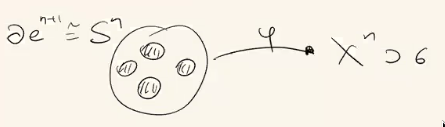
\includegraphics[width=0.8\linewidth]{shaded.png}
        \caption{Diagram of the morphism}%
        \label{fig:shaded}
    \end{figure}
    that the shaded part is $\varphi^{-1}(\sigma^n)$ and $\varphi$ is a homeomorphism on the shaded component. In particular, $f \circ \varphi, g \circ \varphi$ only differ on the shaded part, so the number of components of the shaded part is $[e:\sigma]$.
\end{proof}

\begin{proof}[Proof of fundamental theorem of obstruction theory]
    Let $\mc{O}_f = [c_f] = 0$. Then $c_f = \delta d$ for some $d \in \mc{C}^n(X, \pi_n(Y))$. But then there exists $g \colon X^n \to Y$ such that $\eval{g}_{X^{n-1}} = \eval{f}_{X^{n-1}}$ with $d_{f,g} = -d$. But then 
    \[ c_g = c_f + \delta d_{f,g} = \delta d - \delta d = 0, \]
    so $g$ extends to $X^{n+1}$.

    In the other direction, assume $g \colon X^{n+1} \to Y$ with $\eval{g}_{X^{n-1}} = \eval{f}_{X^{n-1}}$. Therefore $c_g = 0$, and
    \[ c_f = c_f - c_g = - \delta d_{f,g}, \]
    so $[c_f] = 0$.
\end{proof}

Now we will consider the relative case. Suppose $(X, A)$ is a CW-pair and we have $f \colon X^n \cup A \to Y$. Can we extend this to $X^{n+1} \cup A$? Here, we obtain an obstruction class $\mc{O}_f \in H^{n+1}(X, A; \pi_n(Y))$. We have a relative version of the fundamental theorem in this case.

Returning to the homotopy problem, consider $f, g \colon X \to Y$ such that $\eval{f}_{X^{n-1}} \sim \eval{g}_{X^{n-1}}$. Can we extend this homotopy to $X^n$? We are considering the extension problem for
\[ X \times \qty{0} \cup X^{n-1} \times I \cup X \times \qty{1} \subset X \times \qty{0} \cup X^n \times I \cup X \times \qty{1}. \]
We are considering $(n+1)$-cells of the form $e^n \times I$, where $e^n$ is an $n$-cell in $X$. Assume for simplicity that $\eval{f}_{X^{n-1}} = \eval{g}_{X^{n-1}}$. Then the obstruction is \textbf{exactly} $d_{f,g} \in \mc{C}^n(X, \pi_n(Y))$. Also, if $c_f = c_g = 0$, then $\delta d_{f,g} = c_g - c_f = 0$.

\begin{thm}
    Let $f, g \colon X \to Y$ agree on $X^{n-1}$. Then $H^n(X, \pi_n(Y)) \ni [d_{f,g}] = 0$ if and only if $f,g$ are homotopic on $X^n$, with the homotopy fixing $X^{n-2}$.
\end{thm}

\begin{exm}[Cohomology of $K(G, n)$]
    Consider $[X, K(G, n)] \to H^n(X, G)$ by $f \mapsto [d_{f, \text{const}}]$. Here, we can homotope $f$ such that $\eval{f}_{X^{n-1}}$ is constant because $\pi_i(K(G, n)) = 0$ for $i < n$. Surjectivity is obvious from the previous discussion, so we will prove injectivity.

    If $[d_{f, \text{const}}] = 0 \in H^n(X, G)$, then $\eval{f}_{X^n}$ is nullhomotopic. Because $\pi_i(K(G, n)) = 0$ for $i > n$, $f$ is nullhomotopic.
\end{exm}

\section{Primary obstruction class}%
\label{sec:primary_obstruction_class}

We will change our notation. Denote the fiber bundle by $F \hookrightarrow E \to B$. In this new notation, we want to extend a section $s \colon B^n \to E$ to $B^{n+1}$. If $e^{n+1}$ is a cell, then $\eval{E}_{e^{n+1}} \cong e^{n+1} \times F$. We have $s \colon \partial e^{n+1} \to F$ and we want to extend this to $e^{n+1}$. Now we have the map $e^{n+1} \mapsto \mc{C}_s(e^{n+1}) \in \pi_n(F)$. We know that $c_s \in \mc{C}^{n+1}(B, \pi_n(F))$. Now we know $s$ extends to $B^{n+1}$ if and only if $c_s = 0$, $\delta c_s = 0$, and the obstruction class $\mc{O}_s \in H^{n+1}(B, \pi_n(F))$ is zero if and only if $\eval{s}_{B^{n-1}}$ can be extended to $B^{n+1}$.

Now we assume that $F$ is $(n-1)$-connected. Therefore there exists a section $s \colon B^n \to E$ with obstruction class $\mc{O}_s \in H^{n+1}(B, \pi_n(F))$.

\begin{thm}\label{thm:obstA}
    Given $s, s' \colon B^n \to E$, we have $\mc{O}_s = \mc{O}_{s'}$. In particular, this is an \textit{invariant} of the bundle!
\end{thm}

\begin{defn}
    Consider a fiber bundle $\xi \colon F \hookrightarrow E \to B$ with $F$ being $(n-1)$-connected. Then the \textit{primary obstruction class} is defined by be $\mc{O}(\xi) \in H^{n+1}(B, \pi_n(F))$.
\end{defn}

\begin{thm}
    The fiber bundle $\xi$ always admits a section over $B^n$ and it admits a section over $B^{n+1}$ if and only if $\mc{O}(\xi) = 0$.
\end{thm}

\begin{proof}[Proof of Theorem~\ref{thm:obstA}]
    First we note that a homotopy of $s$ does not change $C_s \in \mc{C}^{n+1}(B, \pi_n(F))$. The homotopy extension property holds for sections where $(X, A)$ is a CW pair with $s \colon X \to E$ and $s_t \colon A \times I \to E$ a homotopy of sections. Here, we can extend to $\wt{s}_t \colon X \times I \to E$.

    Now suppose $s, s' \colon B^n \to E$. Of course, $s \sim s'$ on $B^0$. We now show that if $s \sim s'$ on $B^k$, then $s \sim s'$ on $B^{k+1}$ for $0 \leq k < n-1$. To see this, the homotopy extension property tells us that we may assume $s = s'$ on $B^k$ after extending the homotopy. Then, we have $d_{s,s'} \in \mc{C}^{k+1}(B, \pi_{k+1}(F))$. But we see that $d_{s,s'} = 0$, so $s \sim s'$ on $B^{k+1}$. We now obtain $s, s' \colon B^n \to E$ such that $s \sim s'$ on $B^{n-1}$. We may assume that $s = s'$ on $B^{n-1}$. Then we note that $d_{ss'} \in \mc{C}^n(B, \pi_n(F))$, so $c_{s'} - c_s = \delta d_{s,s'}$ and thus $\mc{O}_s = \mc{O}_{s'}$.
\end{proof}

The key property is that if we have $f \colon B' \to B$ and consider the pullback bundle $f^* \xi$, then $\mc{O}(f^* \xi) = f^* \mc{O}(\xi)$. This tells us that $\mc{O}(\xi)$ is a characteristic class, or in other words, a natural cohomological invariant. Consider the basic example: Suppose $\xi \colon S^{n-1} \hookrightarrow E \to B$ is an oriented bundle. Then $S^{n-1}$ is $(n-2)$-connected, so we have an obstruction class $\mc{O}(\xi) \in H^n(B, \Z)$.

\begin{defn}
    This obstruction class is called the \textit{Euler class} $e(\xi)$ of $\xi$. Then $e(\xi) = 0$ if and only if $\xi$ has a section over $B^n$.
\end{defn}

Here we have a special case. If $\eta \colon \R^n \hookrightarrow E \to B$ is an oriented vector bundle and $\xi$ is the associated sphere bundle $S^{n-1} \to S(E) \to B$. Then $e(E)$ is the Euler class of the associated sphere bundle. Therefore $e(E) = 0$ if and only if there exists a nonvanishing section of $\eta$ over $B^n$.

\begin{thm}
    Let $M^n$ be a smooth oriented compact manifold. Then $e(T_M) \in H^n(M, \Z) \cong \Z$ is $\chi(M)$.
\end{thm}

\begin{cor}[Poincare-Hopf]
    $M$ admits a nowhere vanishing vector field if and only if $\chi(M) = 0$.
\end{cor}

\begin{proof}
    Note that $M^{n-1} \cong M \setminus \qty{\text{finite number of points}}$ (one for each top-cell). To compute $\mc{O}(\xi)$ we can use a vector field $v$ with only isolated zeroes. Now we may define the local degree at $x$ to be the degree of the map $S_{\ep} \to S^{n-1}$ defined by $y \mapsto v(y)$. The local degree behaves like 
    \begin{figure}[H]
        \centering
        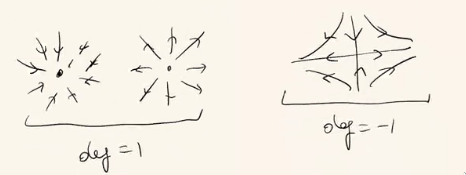
\includegraphics[width=0.8\linewidth]{locdeg}
        \caption{Example of local degrees}%
        \label{fig:locdeg}
    \end{figure}
    and therefore $\Z \ni \mc{O}(\xi) = \sum \text{local degrees}$ by definition. Now we simply need to construct an explicit nice vector field. Because $M$ is smooth, it admits a smooth triangulation.\footnote{Apparently there is also a proof using the Atiyah-Singer index theorem, but that is way more advanced than using this result. Francesco says this is a result everyone uses without knowing the proof.} The vector field is constructed by placing a zero at the center of every face and then for the center of a given positive dimensional face, the vector field points outward towards the vertices of that face. But then we have
    \[ \sum \text{local degrees} = \sum_i \#\qty{\text{$i$-cells}} = \chi(M). \qedhere \]
\end{proof}

\begin{rmk}
    Let $E^k \to M^n$ be a smooth vector bundle with $M$ compact. Then $e(E)$ can be interpreted as follows. Choose a generic section $s \colon M \to E$. Then $s^{-1}(0)$ is a smooth manifold of dimension $n-k$, and so we can write $e(E) = PD(s^{-1}(0))$.
\end{rmk}

We will now relate the primary obstruction class and transgression. We will consider the Serre spectral sequence with coefficients in $\pi_n(F) = H_n(F)$. We know we have the transgression map $\tau \colon H^n(F, \pi_n(F)) \to H^{n+1}(B, \pi_n(F))$ and the fundamental class $\iota \in H^n(F, \pi_n(F))$. This is defined by for all $x \in \pi_n(F), \ev{\iota, h(x)} = x$.

\begin{thm}
    The primary obstruction class is given by $\tau(\iota) = \mc{O}(\xi) \in H^{n+1}(B, \pi_n(F))$.
\end{thm}
Proof of this is given in a series of exercises in Fuchs-Fomenko 23.5.

Now we will consider the \textit{Thom isomorphism}. If $E \to B$ is a rank $n$ vector bundle. Then we may associate the disk bundle $D(E)$ and the sphere bundle $S(E)$. Now we define the \textit{Thom space} to be $T(E) = D(E) / S(E)$ (equivalently, the one-point compactification of $E$).

\begin{thm}[Thom isomorphism]
    Suppose $E$ is an oriented vector bundle. Then there exists a unique $U \in H^n(T(E); \Z) = H^n(D(E), S(E))$ such that $\eval{U}_{\ol{F}}$ is the generator of $H^n(\ol{F}, \Z) = \Z$ (given by orientation). We call $U$ the \textit{Thom class}. Furthermore, we have
    \[ H^k(B, \Z) \cong H^k(D(E); \Z) \xrightarrow{\sim} H^{k+n}(D(E), S(E), \Z) \qquad x \mapsto x \cup U \]
    is an isomorphism for all $k$. Finally, the map 
    \[ H^n(D(E), S(E)) \to H^n(D(E)) \cong H^n(B) \]
    sends the Thom class $U$ to the Euler class $e(E)$.
\end{thm}

\begin{proof}
    Consider the Serre spectral sequence for $(D^n, S^{n-1}) \hookrightarrow (D(E), S(E)) \to B$. Then the Euler class is the Thom class by the prior discussion about transgression. Alternatively, we may construct the Thom class locally and patch, and this can be found in Chapter 10 of Milnor-Stasheff.
\end{proof}

\section{Vector Bundles}%
\label{sec:vector_bundles}

We may consider the functor
\[ \mr{Vect}_{\C}^k \colon \ms{CW}^{\mr{op}} \to \ms{Set} \qquad X \mapsto \qty{\text{rank $k$ complex vector bundles}}. \]
We may also consider the functors $\Vect_{\R}^k, \Vect_{\R}^{+, k}$ of real vector bundles and oriented real vector bundles. This functor is representable!

\begin{thm}[Brown representability]
    Let $h \colon \ms{hCW}_*^{\mr{op}} \to \ms{Set}$ be a functor. If
    \begin{enumerate}
        \item For $X = \bigvee X_{\alpha}$ with $i_{\alpha} \colon X_{\alpha} \hookrightarrow X$, then $\prod i_{\alpha}^* \colon h(X) \simeq \prod h(X_{\alpha})$ is an isomorphism;
        \item If $X = A \cup B$ is a union of subcomplexes and $a \in h(A), b \in h(B)$ retrict to the same element in $h(A \cap B)$, then there exists $x \in h(X)$ restricting to $a,b$,
    \end{enumerate}
    then there exists a CW complex $K$ and $u \in h(k)$ such that 
    \[ [X,k] \to h(X) \qquad f \mapsto f^*(U) \]
    is a bijection.
\end{thm}

Note that for $\Vect_{\C}^k$, the condition of being homotopy invariant is nontrivial to decide. We want $f_t \colon X \times I \to Y$ such that $f_0^* \eta \simeq f_1^* \eta$. The idea is that for $\xi \coloneqq f_t^* \eta \to X \times I$, we need $\eval{\xi}_{X \times 0} = f_0^* \eta, \eval{\xi}_{X \times 1} = f_1^* \eta$.

\begin{prop}
    Let $X$ be a CW complex (or in general $X$ is paracompact). Then if $\xi$ is a vector bundle over $X \times I$, we have $\eval{\xi}_{X \times 0} \simeq \eval{\xi}_{X \times 1}$.
\end{prop}

Recall that $X$ is \textit{paracompact} if $X$ is Hausdorff and any open cover $\qty{U_{\alpha}}$ admits a locally finite refinement $\qty{V_{\beta}}$. This is equivalent to every open cover admitting a partition of unity subordinate to it.

\begin{rmk}
    We may also assume the indices $\beta$ are countable.
\end{rmk}

\begin{exm}
    Any $\eta \to X$ paracompact admits a Hermitian metric. To see this, simply trivialize over the charts $U_{\alpha}$ and then glue using our partition of unity.
\end{exm}

Now we note that if $E \to X \times [a,b]$ is trivial over $[a,c]$ and $[c,b]$, then $E$ is trivial. This implies that any $\eta \to D^k$ is trivial. Fix trivializations $h_1 \colon X \times [a,c] \times \C^k \to E_1$, $h_2 \colon X \times [c,b] \times \C^k \to E_2$. These do not necessarily agree on $X \times \qty{c} \times \C^k$, but we simply consider $\varphi = h_1 h_2^{-1}$ and change $h_2$ by $\varphi$ to get the desired trivialization.

The second observation is that if $\eta \to X \times I$ then there exists an open cover $\qty{U_{\alpha}}$ such that $\eval{\eta}_{U_{\alpha} \times I}$ is trivial. To see this, we simply trivialize over $U_{X,i} \times [t_{i-1}, t_i]$ and then glue the trivializations.

Now we return to the proof that $\Vect_{\C}^k$ is homotopy invariant. Given a partition of unity $\varphi_i$ subordinate to $U_{\alpha}$ (with $\eval{eta}_{U_{\alpha} \times I}$ trivial), we write $\psi_m \colon \varphi_1 + \cdots + \varphi_m \colon X \to [0,1]$. Then define $X_m$ to be the graph of $\psi_m$. We know $\operatorname{supp} \varphi_{m+1} \subseteq U_{\alpha}$ for some $\alpha$, so $p \colon X_{m+1} \to X_m$ lifts to $h_m \colon \eval{\eta}_{X_{m+1}} \to \eval{\eta}_{X_m}$. We know $\eta$ is trivial on $U_{\alpha} \times I$, so we have
\[ h_m(x, \psi_{m+1}(x), v) = (x, \psi_m(x), V). \]
Then we know $X_0$ is $X \times \qty{0}$, so using local finiteness of the partition of unity, we obtain the desired result.

We now want to find a concrete space that represents this functor. Define the \textit{Grassmannian}
\[ G_{n, k}^{\C} = \qty{k\text{-planes in }\C^n} \]
of $k$-planes in $\C^n$. This has a tautological bundle $\C^k \hookrightarrow \gamma_{n, k}^{\C} \to G_{n,k}^{\C}$ given by $\gamma = \qty{(V, v) \mid v \in V}$. Of course, if $m < n$, we know $G_{m,k}^{\C} \hookrightarrow G_{n,k}^{\C}$, so we define $G_k^{\C} \coloneqq G_{\infty,k}^{\C} = \bigcup_n G_{n,k}^{\C}$. Because the tautological bundles are well behaved under this, we obtain a tautological bundle $\gamma_k \to G_k^{\C}$.

\begin{thm}
    The bundle $\gamma_k \to G_k^{\C}$ is a universal bundle. This means that $[X, G_k^{\C}] \simeq \Vect_{\C}^k(X)$, where $f \mapsto f^* \gamma_k$.
\end{thm}

\begin{rmk}
    We can also write $G_k^{\C} = BU(k)$ as the classifying space of $U(k)$.
\end{rmk}

\begin{proof}[Proof of Theorem]
    Let $\eta \to X$. Then $\eta \cong f^* \gamma_k$ if and only if there exists $g \colon \eta \to \C^{\infty}$ which is linear injective on each fiber $\eta_x$. Given $p \colon \eta \to X$, choose a countable cover with $p^{-1}(U_i)$ trivial and $\varphi_i$ a partition of unity subordinate to $U_i$. Then define
    \[ g_i \colon p^{-1}(U_i) = U_i \times \C^n \to \C^n \]
    and consider the map $(\varphi_i \circ p) \cdot g_i \colon \eta \to \C^n$. This defines $g \colon \eta \to {(\C^n)}^{\infty} = \C^{\infty}$.

    Now we need to show that if $g_0, g_1 \colon \eta \to \C^{\infty}$ that are injective on fibers, then there exist $g_t \colon \eta \times I \to \C^{\infty}$ linear injective on fibers at each time. We define
    \[ L_t \colon \C^{\infty} \to \C^{\infty} \qquad (x_1, x_2, \ldots) \mapsto (1-t)(x_1, x_2 \ldots) + t (x_1, 0, x_2, \ldots). \]
    This is injective at each $t$ and moves $g_0$ to the odd entries. Similarly, we can move $g_1$ to the even entries, so we can write $g_t = (1-t) g_0 + t g_1$.
\end{proof}

A \textit{characteristic class} is a natural transformation $\Vect_{\C}^k (X) \xrightarrow{c} H^*(X, \Z)$. By the Yoneda lemma, characteristic classes are in bijection with the cohomology of $G_k^{\C}$. We now study basic facts of the Grassmannians:
\begin{itemize}
    \item There is a transitive action of $U(n)$ on $G_{n,k}^{\C}$. The stabilizer of $\C^k \subset \C^n$ is $U(k) \times U(n-k)$.
    \item Clearly we have $G_{n,1} = \C\P^{n-1}$.
    \item The Grassmannian $G_{n,k}^{\C}$ has a nice cell decomposition generalizing $\C\P^n = \mr{pt} \cup D^2 \cup D^4 \cup D^6 \cup \cdots$.
\end{itemize}

\begin{exm}
    Consider the Grassmannian $G_{4,2}$ of $2$-planes in $\C^4$. Then the interior of cells is described by dimensions of intersections with $\C^1 \subset \C^2 \subset \C^4 \subset \C^4$. The cells are given by:
    \begin{description}
        \item[$0$-cell:] This is just $\qty{\C^2}$ corresponding to $(1,2,2)$.
        \item[$2$-cell:] This is the set $\qty{\C^1 \subset V \subset \C^3}$ corresponding to $(1,1,2)$.
        \item[$4$-cells:] These are $\qty{\C^1 \subset V}$ corresponding to $(1,1,1)$ and $\qty{V \subset \C^3}$ corresponding to $(0,1,2)$.
        \item[$6$-cell:] This is given by $\qty{\dim V \cap \C^2 > 0}$ corresponding to $(0,1,1)$.
        \item[$8$-cell:] This is everything else, which corresponds to $(0,0,1)$.
    \end{description}
\end{exm}

For an alternative description, a $2$ plane corresponds to the row reduced echelon form of a $2 \times 4$ matrix. Then we have the following correspondence:
\begin{description}
    \item[$0$-cell:] This is the matrix $\mqty[ 0 & 0 & 1 & 0 \\ 0 & 0 & 0 & 1 ]$.
    \item[$2$-cell:] This is the matrix $\mqty[ 0 & 1 & * & 0 \\ 0 & 0 & 0 & 1 ]$.
    \item[$4$-cells:] These are the matrices $\mqty[ 1 & * & * & 0 \\ 0 & 0 & 0 & 1 ], \mqty[ 0 & 1 & 0 & * \\ 0 & 0 & 1 & * ]$.
    \item[$6$-cell:] This is the matrix $\mqty[ 1 & * & 0 & * \\ 0 & 0 & 1 & * ]$.
    \item[$8$-cell:] This is the matrix $\mqty[ 1 & 0 & * & * \\ 0 & 1 & * & * ]$.
\end{description}
These cells are called \textit{Schubert cells}. These behave nicely with the inclusions and $G_{n,k}$ has $\binom{n}{k}$ cells. The number of $2i$-cells is given by the number of partitions of $i$ into at most $k$ integers that are each at most $n-k$. The cells are of even dimension, so we can compute the group structure on the cohomology, but not the ring structure.

\begin{thm}
    The ring struction on cohomology of the Grassmannian is given by $H^*(G_k^{\C}, \Z) \cong \Z[c_1, \ldots, c_k]$, where $\deg c_i = 2i$.
\end{thm}

\begin{defn}
    The characteristic classes of $E \to B$ associated to the $c_i$ are the \textit{Chern classes} $c_i(E)$. By convention, $c_j(E) = 0$ for $j > \dim E$.  
\end{defn}

\begin{proof}
    We need many fibrations. Consider the spaces $G_{n,k}$ of $k$-planes in $\C^n$ and $F_{n,k}$ of $k$-flags in $\C^n$. It is clear that $F_{n,k}$ also parameterizes ordered $k$-tuples of orthogonal complex lines. Of course there is a fibration $F_{k, k} \hookrightarrow F_{n,k} \to G_{n,k}$. We can also understand $H^*(G_k^{\C})$ inductively as well.

    Now we will show that $H^*(F_{\infty,k}) \cong \Z[x_1, \ldots, x_k]$, where $\deg x_i = 2$. Each $x_i$ is the pullback of the generator of $H^2(\C\P^{\infty})$ under the maps $(\ell_1, \ldots, \ell_k) \mapsto \ell_i$. We will use the fibration $\C\P^{n-k} \hookrightarrow F_{n,k} \to F_{n,k-1}$. By induction, we have a fibration
    \[ \C\P^{\infty} \hookrightarrow F_{\infty, k} \to F_{\infty, k-1} \]
    and $H^*(F_{\infty}, k-1) \cong \Z[x_1, \ldots, x_{k-1}]$. Now we use the Leray-Hirsch theorem, but first we need to show that $H^*(E) \twoheadrightarrow H^*(F)$. This is because we have the map $F_{\infty, k} \to \C\P^{\infty}$ given by $(\ell_1, \ldots, \ell_k) \to \ell_k$ and this restricts to the generator of $\C\P^{\infty}$ udner $\C\P^{\infty} \hookrightarrow F_{\infty, k}$. Therefore, $H^*(F_{\infty,k})$ is a free $\Z[x_1, \ldots, x_{k-1}]$-module with additive basis $1, x_k, x_k^2, \ldots$. Now we observe that 
    \[ F_{\infty, k} \hookrightarrow {(\C\P^{\infty})}^k \]
    is a homotopy equivalence by Hurewicz.

    Now we need to consider the fibration $F_{k,k} \hookrightarrow F_{\infty, k} \xrightarrow{\rho} G_{\infty, k}$. This induces a surjective map in cohomology, so by Leray-Hirsch, $H^*(F_{\infty}, k)$ is a free $H^*(G_{\infty}, k)$-module with basis $1, \ldots$ and thus $\rho^* \colon H^*(G_{\infty, k}) \to H^*(F_{\infty, k})$ is injective. The map $F_{\infty, k} \to G_{\infty, k}$ sends a $k$-tuple of lines to their sum. We also know that $\rho$ is $S_k$-invariant, so on cohomology, we have an injection
    \[ H^*(G_{\infty}, k) \hookrightarrow {H^*(F_{\infty,k})}^{S_k} = {\Z[x_1, \ldots, x_k]}^{S_k} = \Z[\sigma_1, \ldots, \sigma_k], \]
    where $\sigma_i$ is the $i$th elementary symmetric polynomial. But then by a dimension count, this injection is surjective.
\end{proof}

\begin{thm}[Splitting principle]
    Let $E^n \to X$ be a line bundle. Then there exists $\wt{X} \xrightarrow{f} \to X$ such that $f^* E$ is a direct sum of line bundles and $f^* \colon H^*(X, \Z) \to H^*(\wt{X}, \Z)$ is injective.
\end{thm}
This gives us the following slogan:
\begin{quotation}
    \textit{When working with Chern classes, we can assume $E$ is a direct sum of line bundles $E \cong L_1 \oplus \cdots \oplus L_k$.} 
\end{quotation}

\begin{proof}
    Set $\wt{X} = F_k(E) \to X$. Then the fiber over $x \in X$ is the space of $k$-flags in $E_x$. Therefore we have a fibration $F_{k,k} \hookrightarrow \wt{X} \to X$. Now $\wt{X}$ has a tautological splitting, where over the point $(\ell_1, \ldots, \ell_k)$ we have the vector space $\ell_1 \oplus \cdots \oplus \ell_k = E_x$. This pulls back $E$ as a direct sum of line bundles.
\end{proof}

Now here are some properties of Chern classes:
\begin{enumerate}
    \item For any $E$, we have $c_0(E) = 1$.
    \item If $\gamma$ is the tautological bundle over $\C\P^1$, then $c_1(\C\P^1) = -x$ and thus $\gamma = \mc{O}(-1)$.
    \item For vector bundles $E, F$, we have $C_k(E \oplus F) = \sum c_k(E) \cup C_{k-i}(F)$. Equivalently, if we define the Chern class $c(E) = 1 + c_1(E) + c_2(E) + \cdots$, then $c(E \oplus F) = c(E) c(F)$.
\end{enumerate}

\begin{proof}
    We prove this for the universal bundles. We have the bundle $\gamma_k \times \gamma_{\ell}$ over $G_k \times G_{\ell}$, and this is given by a classifying map $G_k \times G_{\ell} \to G_{k + \ell}$. Now under the map ${(\C\P^{\infty})}^k \times {(\C\P^{\infty})}^{\ell} \to G_k \times G_{\ell}$, we know $\gamma_k \times \gamma_{\ell}$ pulls back to a direct sum of tautological bundles, and the same is true for $\gamma_{k+\ell}$ pulled back to ${(\C\P^{\infty})}^{k + \ell}$. Therefore, we have
    \[ c(\gamma_{k + \ell}) = (1 + x_1) \cdots (1 + x_k) (1 + y_1) \cdots (1 + y_{\ell}) = c(\gamma_k) c(\gamma_{\ell}). \qedhere \]
\end{proof}

In fact, the three properties determine the $\qty{c_i}$ uniquely.

\begin{rmk}
    \begin{itemize}
        \item If $\C$ is the trivial bundle, then $c_i(E \oplus \C) = c_i(E)$.
        \item If $\ol{E}$ is the complex conjugate bundle of $E$, then $c_i(\ol{E}) = {(-1)}^i c_i(E)$. Note that this is also the dual bundle.
    \end{itemize}
\end{rmk}

\begin{exm}
    We have $c(T \C\P^n) = {(1+x)}^{n+1} = 1 + nx + \binom{n}{2} x^2 + \cdots \in \Z[x]/x^{n+1}$. To describe this, we consider the tautological bundle $\gamma \to \C\P^{n+1}$. Clearly $T_L \C\P^n = \Hom_{\C}(L, L^{\perp})$, where the perp is taken in $\C^{n+1}$. Therefore, $T \C\P^n \equiv \Hom_{\C}(\gamma, \gamma^{\perp})$ and $\gamma \oplus \gamma^{\perp} = \C^{n+1}$. This gives us
    \begin{align*}
        T \C\P^n \oplus \C &\cong \Hom(\gamma, \gamma^{\perp}) \oplus \Hom(\gamma, \gamma) \\
                           &= \Hom(\gamma, \C^{n+1}) \\
                           &= {\Hom(\gamma, \C)}^{n+1} = {\mc{O}(1)}^{n+1}
    \end{align*}
    and therefore 
    \[ c(T\C\P^n) = c(T\C\P^n \oplus \C) = {c(\mc{O}(1))}^{n+1} = {(1+x)}^{n+1}. \]
\end{exm}

We will now consider Chern classes as obstructions. Let $\C^n \hookrightarrow E \to B$ be a rank $n$ bundle. Then we can take orthonormal frames to obtain $V_{n, k}^{\C} \hookrightarrow V_k(E) \to B$. Then sections of $V_k(E) \to B$ are $k$-tuples of sections of $E$ which are orthonomal at each point.

\begin{lem}
    We have
    \[ \pi_i(V_{n,k}^{\C}) = \begin{cases}
        0 & i \leq 2 (n-k) \\
        \Z & i = 2(n-k) + 1.
    \end{cases} \]
\end{lem}

Therefore, the first obstruction to finding a section of $V_k(E)$ over the $2(n-k) + 2$ skeleton lives in $H^{2(n-k)+2}(B, \Z)$. In fact, this is the Chern class. The Chern class $c_j(E) \in H^{2j}(B, \Z)$ is the obstruction to finding $k = (n+1-j)$ linearly independent sections over the $2(n+1-j)$-skeleton. Now observe that $V_{n,1} = S^{2n-1}$. Therefore, if $\dim_{\C} E = n$, we have $c_n(E) = e(E)$.

\section{Real Vector Bundles}%
\label{sec:real_vector_bundles}

Now consider a vector bundle $\R^n \hookrightarrow E \to B$.

\begin{lem}
    For $i < n-k$, we have $\pi_n(V_{n,k}^{\R}) = 0$. In addition, 
    \[ \pi_{n-k}(V_{n,k}^{\R}) = \begin{cases}
        \Z & k=1 \text{ or } n-k \text{ even. } \\
        \Z_2 & \text{otherwise}.
    \end{cases} \]
\end{lem}
Therefore we obtain obstruction classes $\mc{O}_i \in H^i(B, \wt{Z})$ or $\mc{O}_i \in H^i(B, \Z_2)$. This is an obstruction to finding $n+1-i$ linearly independent sections on the $i$-skeleton. Reducing everything modulo $2$, we have
\begin{defn}
    The \textit{Stiefel-Whitney classes} of $E$ are defined by $w_i \coloneqq \mc{O}_i \mod 2$.
\end{defn}
Here are some facts about the Stiefel-Whitney classes:
\begin{itemize}
    \item If $\gamma \to \R\P^1$ is the tautological class, then $w_1(\gamma) = 1 \in H^1(\R\P^1, \Z_2)$.
    \item These correspond to $H^*(G_k^{\R}; \Z_2) = \Z_2[w_1, \ldots, w_k]$, where $\abs{w_i} = i$. Note that it is harder to compute the cohomology in this case than in the complex case.
    \item We have $w_1(E) = 0$ if and only if $E$ is orientable.
    \item If $\dim E = n$ and $E$ is orientable, then $w_n(E) = e(E) \mod 2$.
    \item They are related to $\Sq^{\bullet}$ on $T(E)$ (and in fact this is the definition given in Milnor-Stasheff).
\end{itemize}

Now we will assume that our real vector bundles are oriented. Recall that $G_k^{\R} = BO(k)$ is the space of $k$-planes in $\R^{\infty}$. Then we set $G_k^+ = BSO(k)$ to be the space of \textbf{oriented} $k$-planes in $\R^{\infty}$. There is a double cover $G_k^+ \to G_k^{\R}$. Recall that every oriented bundle has an Euler class!
\begin{rmk}
    Suppose $E \to B$ os an oriented odd-dimensional vector undle. Then the map $(b, v) \mapsto (b,-v)$ reverses orientation on the sphere bundle, so $e(E) = -e(E)$ and thus $2e(E) = 0$.
\end{rmk}

Recall that $H^*(SO(n), \Q)$ varies greatly depending on the parity of $n$. We should obtain the same thing for the classifying spaces.

\begin{thm}
    Over $\Q$, we have $H^*(G_{2m+1}^+) \Q[p_1, \ldots, p_m]$, where $\abs{p_i} = 4i$. In the even case, we have $H^*(G_{2m}^+) = \Q[p_1, \ldots, p_m, e]/(e^2=p_m)$.
\end{thm}
We are mostly interested in even-dimensional manifolds, so we will mostly work in the second case.

\begin{defn}
    The characteristic classes corresponding to $p_1, \ldots, p_m$ are called the \textit{Pontryagin classes} of $E$. 
\end{defn}

Concretely, we can define the Pontryagin classes in terms of the Chern classes. If $E \to B$ is a real vector bundle, we may take $E \otimes \C \to B$ the corresponding complex vector bundle. Then we have
\[ p_i(E) \coloneqq {(-1)}^i c_{2i}(E \otimes \C) \in H^{4i}(B, \Z). \]

\begin{rmk}
    Recall that $E \otimes \C$ is always isomorphic to its dual. Complex conjugation gives an antilinear involution, so $c_{2i+1}$ is $2$-torsion.
\end{rmk}

\begin{exm}
    We will compute the Pontragin classes of $T\C\P^n$.
\end{exm}

\begin{lem}
    If $E$ is already a complex vector bundle, then $E \otimes \C \cong E \oplus E^*$ as complex vector bundles.
\end{lem}

\begin{proof}
    Define by $i$ the complex structure on $E$. Then the map $(v,0) \mapsto (v,-iv), (0,w) \mapsto (w,iw)$ is a $\C$-linear isomorphism.
\end{proof}

In particular, if $E$ is complex, then the \textit{total Pontryagin class} $p(E) = 1 + p_1(E) + p_2(E) + \cdots$ can be computed using
\begin{align*}
    1 - p_1(E) + p_2(E) - p_3(E) + \cdots &= 1 + c_2(E \otimes \C) + c_4(E \otimes \C) + c_6(E \otimes \C) \\
                                          &= c(E \otimes \C) \\
                                          &= c(E \oplus E^*) \\
                                          &= c(E) \cdot c(E^*) \\
                                          &= (1 + c_1(E) + c_2(E) + \cdots) (1-c_1(E) + c_2(E) - c_3(E) + \cdots).
\end{align*}
For $T\C\P^n$, we have
\begin{align*}
    1 - p_1 + p_2 - p_3 + \cdots &= {(1+x)}^{n+1} {(1-x)}^{n+1} \\
                                 &= {(1-x^2)}^{n+1},
\end{align*}
so we obtain
\[ p_k(\C\P^n) = \binom{n+1}{k} a^{2k}. \]

Now we will consider Pontryagin roots. The splitting principle for $E^{2m} \to B$ says that $E$ can always be thought of as a direct sum of oriented $2$-plane bundles analogously to Chern classes. Note that an oriented $2$-plane bundle is the same as a complex line bundle (because $i$ rotates by $\frac{\pi}{2}$ counterclockwise). In the case where we actually have $E = L_1 \oplus L_2 \oplus \cdots \oplus L_n$, we obtain
\[ E \otimes \C = L_1 \oplus L_1^* \oplus L_2 \oplus L_2^* \oplus \cdots \oplus L_m \oplus L_m^*. \]
These have Chern roots $\pm x_1, \pm x_2, \ldots, \pm x_m$, so we have
\begin{align*} 
    p_1(E) &= -c_2(E \otimes \C) = x_1^2 + x_2^2 + \cdots + x_m^2 \\
    p_2(E) &= \sigma_2(x_1^2, \ldots, x_m^2) \\
    \vdots & \\
    p_m(E) &= x_1^2 x_2^2 \cdots x_m^2 = \sigma_m(x_1^2, \ldots, x_m^2).
\end{align*}
This tells us that the $x_i^2$ are the Pontryagin roots. Also, $e(E) = x_1 \cdots x_m$, so $e^2 = p_m$.

\begin{rmk}
    This is related to the fact that $\det \colon \mf{so}(2m) \to \R$ has an $SO(2m)$-invariant square root, called the \textit{Pfaffian}.
\end{rmk}

\subsection{Relation to Steenrod problem and oriented bordism}%
\label{sub:relation_to_steenrod_problem_and_oriented_bordism}

Let $X^n$ be a closed smooth manifold and $\alpha \in H_k(X, \Z)$.
\begin{quest}
    Is there an oriented smooth manifold $M^k$ and continuous $f \colon M \to X$ such that $f_*[M] = \alpha$?
\end{quest}

\begin{defn}
    A pair $(M, f)$ is \textit{singular manifold} representing $\alpha$.
\end{defn}

Now define 
\[ \Omega_k(X) \coloneqq \frac{ \qty{(M^k, f)\ \text{singular manifold in $X$}} }{\qty{(M, f) \mid \text{there exists }\partial W = M, f\ \text{extends to $W$}}} \]
with addition given by disjoint union. In addition, we set $-[M, f] = [\ol{M}, f]$. This is well-defined, and in fact there is a map
\[ \Omega_n(X) \to H_n(X, \Z) \qquad [(M, f)] \mapsto f_*[M]. \]
The group $\Omega_k(X)$ is called the $k$-th \textit{bordism group}. Clearly $\Omega_k$ is functorial by postcomposition.

\begin{rmk}
    The functors $\Omega_*$ give a generalized homology theory. Note that $\Omega_k(\mr{pt})$ is very complicated. These are given by
    \[ \Omega_k(\mr{pt}) = \frac{\qty{M^k \text{ oriented $k$-manifolds}}}{\qty{M = \partial W^{k+1}}}. \]
\end{rmk}

\begin{thm}
    If $M^{4k} = \partial W^{4k+1}$, then the signature of $M$ is $0$.
\end{thm}

\begin{exm}
    In $\Omega_{4k}(\mr{pt})$, $[\C\P^{2k}] \neq 0$.
\end{exm}

\begin{lem}
    If $B \colon V \otimes V \to \R$ is symmetric and nondegenerate and $W \subset V$ is isotropic and $\dim W = \frac{1}{2} \dim V$, then the signature of $B$ is $0$.
\end{lem}

\begin{rmk}
    Actually, it is easy to see that $B = \begin{psmallmatrix}
        0 & W \\ 1 & 0
    \end{psmallmatrix}^{\oplus \dim W}$.
\end{rmk}

\begin{lem}
    Let $\iota \colon M \hookrightarrow W$ be the inclusion onto the boundary. Then $\ev{\iota^*(c), [M]} = 0$ for all $c \in H^{4k}(W)$.
\end{lem}

\begin{proof}
    This is given by $\ev{i^*(c), [M]} = \ev{c, i_* [M]} = 0$ because in the exact sequence 
    \[ H_{4k+1}(W, M) \xrightarrow{\delta} H_{4k}(M) \xrightarrow{\iota_*} H_{4k}(W),\]
    we have $[W.M] \mapsto [M]$, so $[M] = 0$.
\end{proof}

\begin{proof}[Proof of Theorem]
    Consider the commutative diagram
    \begin{equation*}
    \begin{tikzcd}
        H^{2k}(W) \ar{r}{\iota^*} \ar[equal]{d} & H^{2k}(M) \ar[equal]{d} \ar{r} & H^{2k+1}(W, M) \ar[equal]{d} \\
        H_{2k+1}(W, M) \ar{r} & H_{2k}(M) \ar{r}{\iota_*} & H_{2k}(W).
    \end{tikzcd}
    \end{equation*}
    We know that $W = \Im(\iota^* \colon H^{2k}(W) \to H^{2k}(M))$ is isotropic in $V = H^{2k}(M)$, so we need to show that it is half-dimensional. But then $\Im(\iota^*) = \ker (\iota_*)$ under identification. But then $\iota^*$ is dual to $\iota_*$, so $\dim \Im(\iota^*) = \dim \Im(\iota_*) = \dim V - \dim \ker (\iota_*)$ and thus $W$ is half-dimensional.
\end{proof}








\end{document}
